\documentclass[12pt]{article}
\usepackage{times} 			% use Times New Roman font

\usepackage[margin=1in]{geometry}   % sets 1 inch margins on all sides
\usepackage{hyperref}               % for URL formatting
\usepackage[pdftex]{graphicx}       % So includegraphics will work
\setlength{\parskip}{1em}           % skip 1em between paragraphs
\usepackage{indentfirst}            % indent the first line of each paragraph
\usepackage{datetime}
\usepackage[small, bf]{caption}
\usepackage{listings}               % for code listings
\usepackage{xcolor}                 % for styling code
\usepackage{multirow}

%New colors defined below
\definecolor{backcolour}{RGB}{246, 246, 246}   % 0xF6, 0xF6, 0xF6
\definecolor{codegreen}{RGB}{16, 124, 2}       % 0x10, 0x7C, 0x02
\definecolor{codepurple}{RGB}{170, 0, 217}     % 0xAA, 0x00, 0xD9
\definecolor{codered}{RGB}{154, 0, 18}         % 0x9A, 0x00, 0x12

%Code listing style named "gcolabstyle" - matches Google Colab
\lstdefinestyle{gcolabstyle}{
  basicstyle=\ttfamily\small,
  backgroundcolor=\color{backcolour},   
  commentstyle=\itshape\color{codegreen},
  keywordstyle=\color{codepurple},
  stringstyle=\color{codered},
  numberstyle=\ttfamily\footnotesize\color{darkgray}, 
  breakatwhitespace=false,         
  breaklines=true,                 
  captionpos=b,                    
  keepspaces=true,                 
  numbers=left,                    
  numbersep=5pt,                  
  showspaces=false,                
  showstringspaces=false,
  showtabs=false,                  
  tabsize=2
}

\lstset{style=gcolabstyle}      %set gcolabstyle code listing

% to make long URIs break nicely
\makeatletter
\g@addto@macro{\UrlBreaks}{\UrlOrds}
\makeatother

% for fancy page headings
\usepackage{fancyhdr}
\setlength{\headheight}{13.6pt} % to remove fancyhdr warning
\pagestyle{fancy}
\fancyhf{}
\rhead{\small \thepage}
\lhead{\small HW 5\, Venkatesh}  % EDIT THIS, REPLACE # with HW number
\chead{\small CS 532, Fall 2021} 

%-------------------------------------------------------------------------
\begin{document}

% EDIT THE ITEMS HERE
\begin{centering}
{\large\textbf{HW 5\ - Graph Partitioning}}\\ 
Swathi Venkatesh\\
11/14/2021\\
\end{centering}

%-------------------------------------------------------------------------

% The * after \section just says to not number the sections
\section*{Q1}
Draw the original Karate club graph (before the split) and color the nodes according to the factions they belong to (John A or Mr. Hi). This should look similar to the graph on slide 92 - all edges should be present, just indicate the nodes in the eventual split by color.

\subsection*{Answer}

%Python code highlighting
\begin{lstlisting}[language=Python, caption=mygraph.py , label=lst:copy]
import re
import numpy as np
import networkx as net
import matplotlib.pyplot as plt

def color(p,f,lst):
    col = []
    lent = len(p)
    if f == "" and len(lst) ==0:
        col = ['yellow'] * 34
        col[0] = "red"
        col[33] = "green"        
    elif(f=="final" and len(lst) == 2):
        
        col = ['blue'] * 34
        for n in lst[0]:
            col[n] = "red"  
        for t in lst[1]:
            col[t] ="green"
    return col

def findedge(G0): 
    """
    The edge_betweenness in a networkx returns dictionary.
    Which is then made to a list; sorted and it returns edge with highest betweenness
    """
    betweenness = net.edge_betweenness_centrality(G0)
    betweenness_li = list(betweenness.items())
    betweenness_li.sort(key=lambda z: z[1], reverse=True)
    return betweenness_li[0][0]

def component(G):
    if len(G.nodes()) == 1:
        return [G.nodes()]
    comp = (G.subgraph(c) for c in net.connected_components(G))
    comp = list(comp)
    cnt = 0
    while len(comp) == 1:
        cnt +=1
        G.remove_edge(*findedge(G))
        
        comp =(G.subgraph(c) for c in net.connected_components(G))        
        comp = list(comp)
    return comp

def graph(G, color, path,empty,edgecl_map,wei_map):
    string = re.search(r'((q[0-9]\/)([0-9a-zA-z]*\.png))',path)
    name = string.group(3)
    plt.figure(figsize=(15,8.8))
    if empty == "":
        net.draw_kamada_kawai(G,with_labels=True, node_color = color)
    else:
        
        pos = net.spring_layout(G, k=0.3*1/np.sqrt(len(G.nodes())) +0.1, iterations=20)
        net.draw(G,with_labels=True ,node_color = color,pos=pos,edge_color=edgecl_map,width = list(wei_map))

    plt.savefig(path, format="PNG")
    plt.show()
    plt.close()
    return 0

def coloredges(G,tuplesEdgeToRemove,reset):
    """
    This builds the edge attributes color and weight
    """
    tot = G.number_of_edges()
    coloredge_map = ['black'] * tot
    wei_map = [1.5] * tot
    if(reset =="n"):
        tot = -1
        for n in G.edges:
            tot += 1
            if tuplesEdgeToRemove == n:
                coloredge_map[tot] = 'blue'
                wei_map[tot] = 3.2
    return coloredge_map,wei_map

def girvannewman_graph(G):
    comp = (G.subgraph(c) for c in net.connected_components(G))
    comp = list(comp)
    c =0
    while len(comp) == 1:
        c +=1
        path = "q2/" +str(c) +"x.png"
        #find the best edge and return as a list
        bestedge = findedge(G)
        edgecolor,weightMap = coloredges(G, bestedge,"n")
        graph(G,col,path,"spacing",edgecolor,weightMap)
        #Remove the best edge
        G.remove_edge(*bestedge)
        #ReSet everything back to black and reset the weight too
        edgecolor,weightMap = coloredges(G, bestedge,"")
        path = "q2/" + str(c) +"y.png"
        
        graph(G,col,path,"spacing",edgecolor, weightMap)
        
    return 0
try:
    k = net.karate_club_graph()
    t = k
    """
    Got the data from networkx
    parsed the data to assign colorcoding for the two main leaders
    then plotted the graph
    """
    k = net.karate_club_graph()
    col = color(k, "","")
    graph(k,col, "q1/karate.png","","","")
    """
    passed the retrieved data to the Girvan newman algorithm
    color coded the result of the splitted group
    then plotted the graph
    """
    final = component(k)
    #Set the colors based on the list received
    col = color(k,"final",final)
    graph(k,col,"q1/finalgroup.png","","","")
    girvannewman_graph(t)
except Exception as e:
    print(e)
\end{lstlisting}



\begin{figure}[h]
    \centering
    % trim and clip are used to crop the image, trim=left bottom right top
    % width sets max width, height will be scaled appropriately
    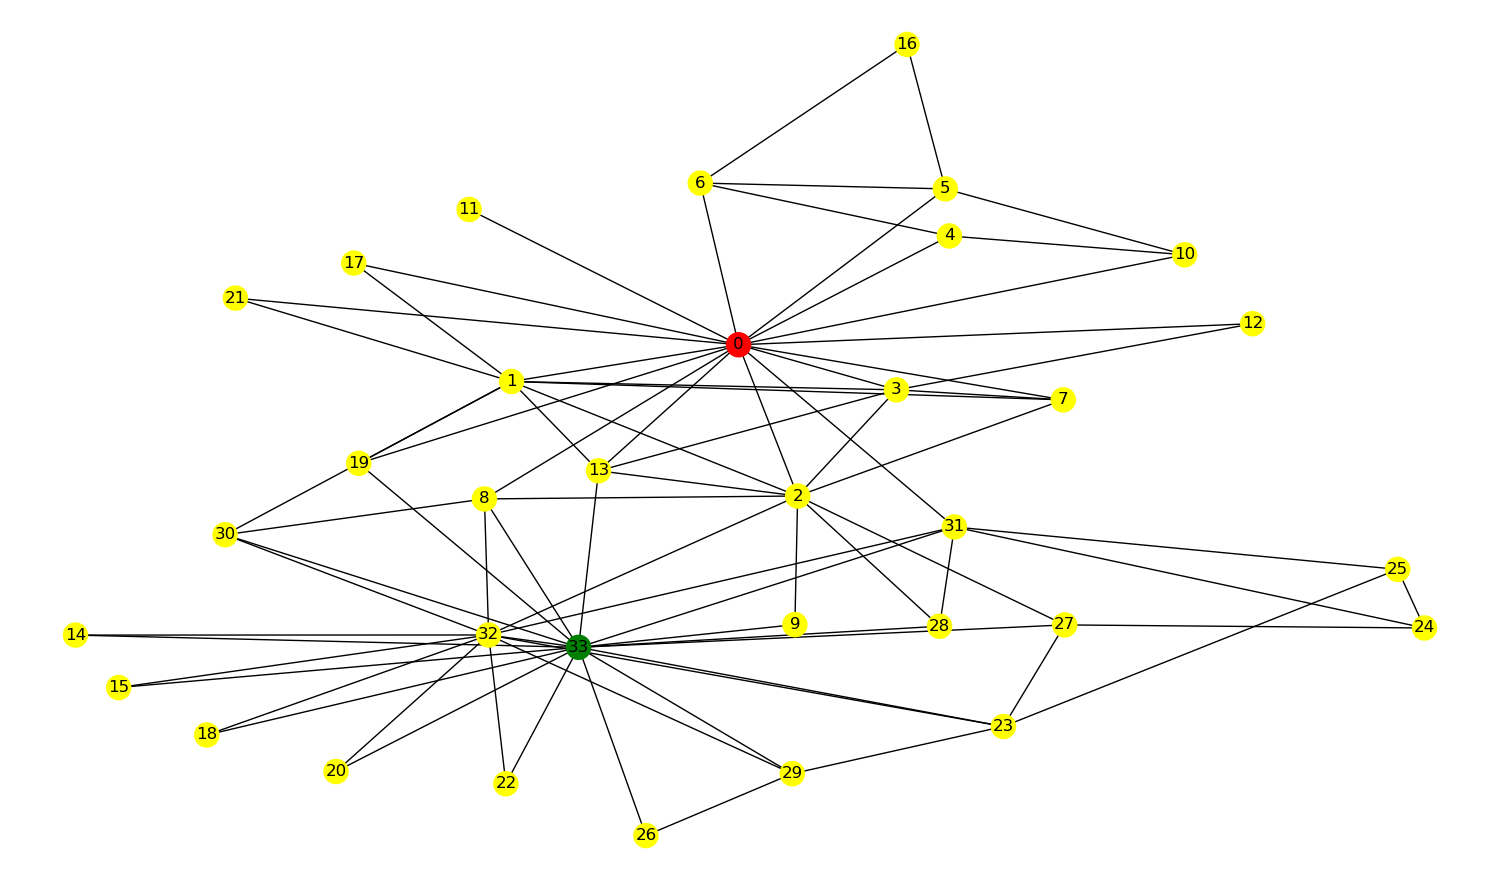
\includegraphics[trim=0 8 0 0, clip, width=170mm,scale=0.5] {karate.PNG}
    \caption{Dataset having two groups Red: John A and Green: Mr.Hi and yellow for others }
    \label{fig:web-growth}
\end{figure}

\begin{figure}[h]
    \centering
    % trim and clip are used to crop the image, trim=left bottom right top
    % width sets max width, height will be scaled appropriately
    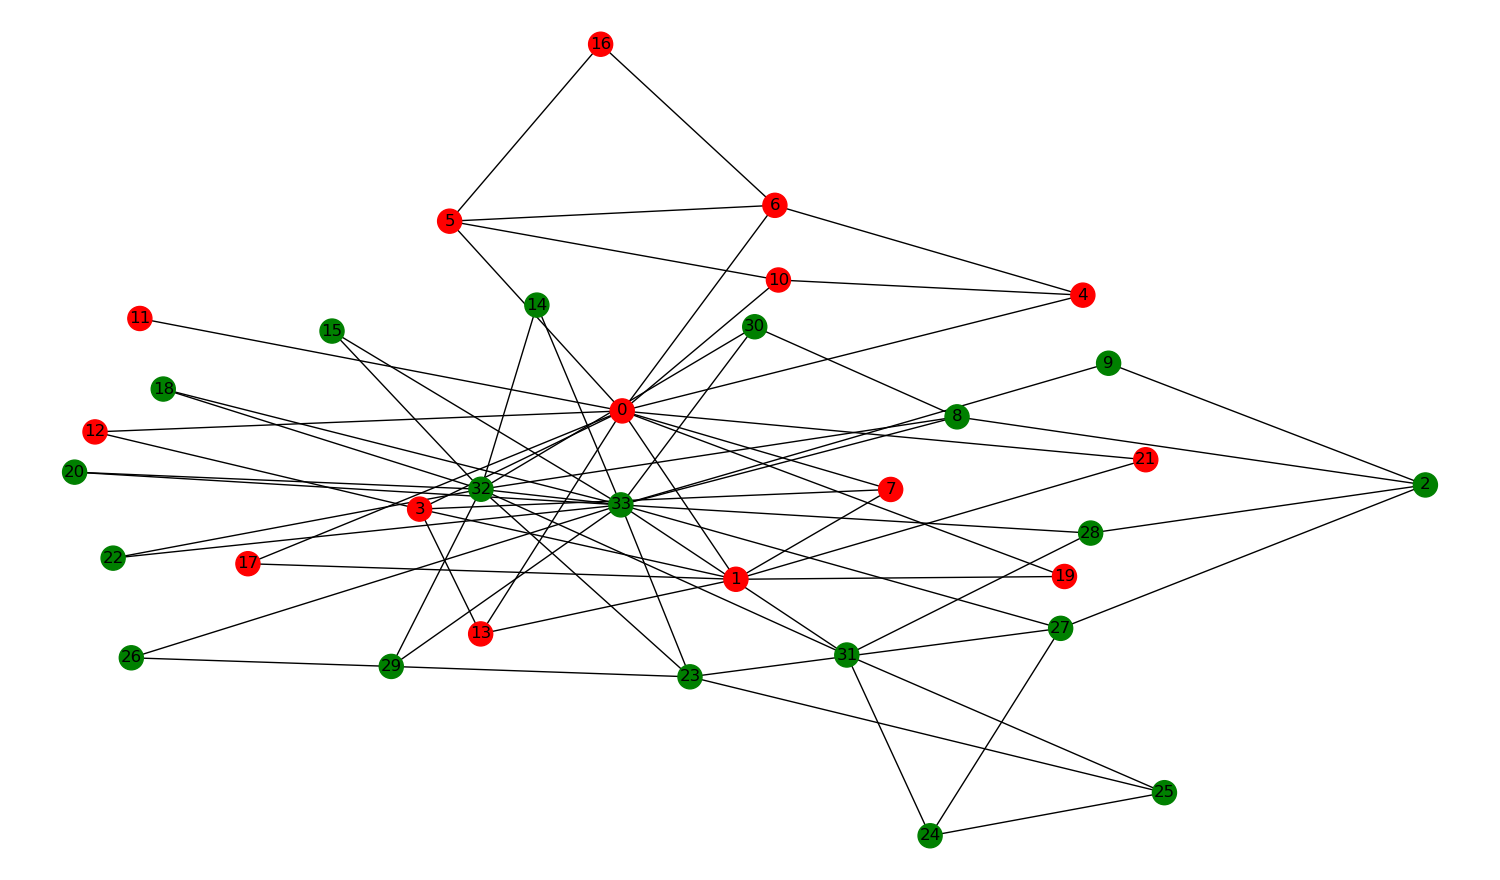
\includegraphics[trim=8 0 8 8, clip, width=170mm] {finalgroup.PNG}
    \caption{Appropriately divided node colors but edges are same}
    \label{fig:web-growth}
\end{figure}

\clearpage
\subsection*{Discussion}
I used networkx library. For this graph, I highlighed the two major parts of the Zachary karate club, John A which represents the Red color and node number 0, while Mr Hi represent the color green and node number 33. 
\begin{itemize}
        \item The driver for the question \lstinputlisting[language=Python,caption=mygraph.py, label=Q1:import,firstnumber=106,firstline=106,lastline=108]{mygraph.py}
        \item The color function builds the list of the color for each nodes 
        \lstinputlisting[language=Python,caption=Building list for the color node in the graph, label=Q1:import,firstnumber=6,firstline=6,lastline=20]{mygraph.py}
        \item A graphing function is used for graphing the data. 
         \lstinputlisting[language=Python,caption= Making the plot for all the graphs (snapshot in mygraph.py), label=Q1:import,firstnumber=46,firstline=46,lastline=60]{mygraph.py}
\end{itemize}
\emph{Q: How many nodes eventually go with John and how many with Mr. Hi?}

 Out of 34 nodes 17 nodes belong to John A and other 17 belong to Mr. Hi
\section*{Q2}
Keeping the node colors the same as they were in Q1, run multiple iterations of the Girvan-Newman graph partioning algorithm (see Module-07 Social Networks, slides 90-99) on the Karate Club graph until the graph splits into two connected components. Include an image of the graph after each iteration in your report.

Note that you will have to implement the Girvan-Newman algorithm rather than relying on a built-in function, as a built-in function will automatically run the whole algorithm and you will not be able to view the intermediate graphs. Make sure that you explain in your report what the Girvan-Newman algorithm is doing.
\subsection*{Answer}
\lstinputlisting[language=Python,caption=Girvan-newman algorithm (snapshot from mygraph.py), label=Q2:import,firstnumber=78,firstline=78,lastline=97]{mygraph.py}

\begin{figure}[h]
    \centering
    % trim and clip are used to crop the image, trim=left bottom right top
    % width sets max width, height will be scaled appropriately
    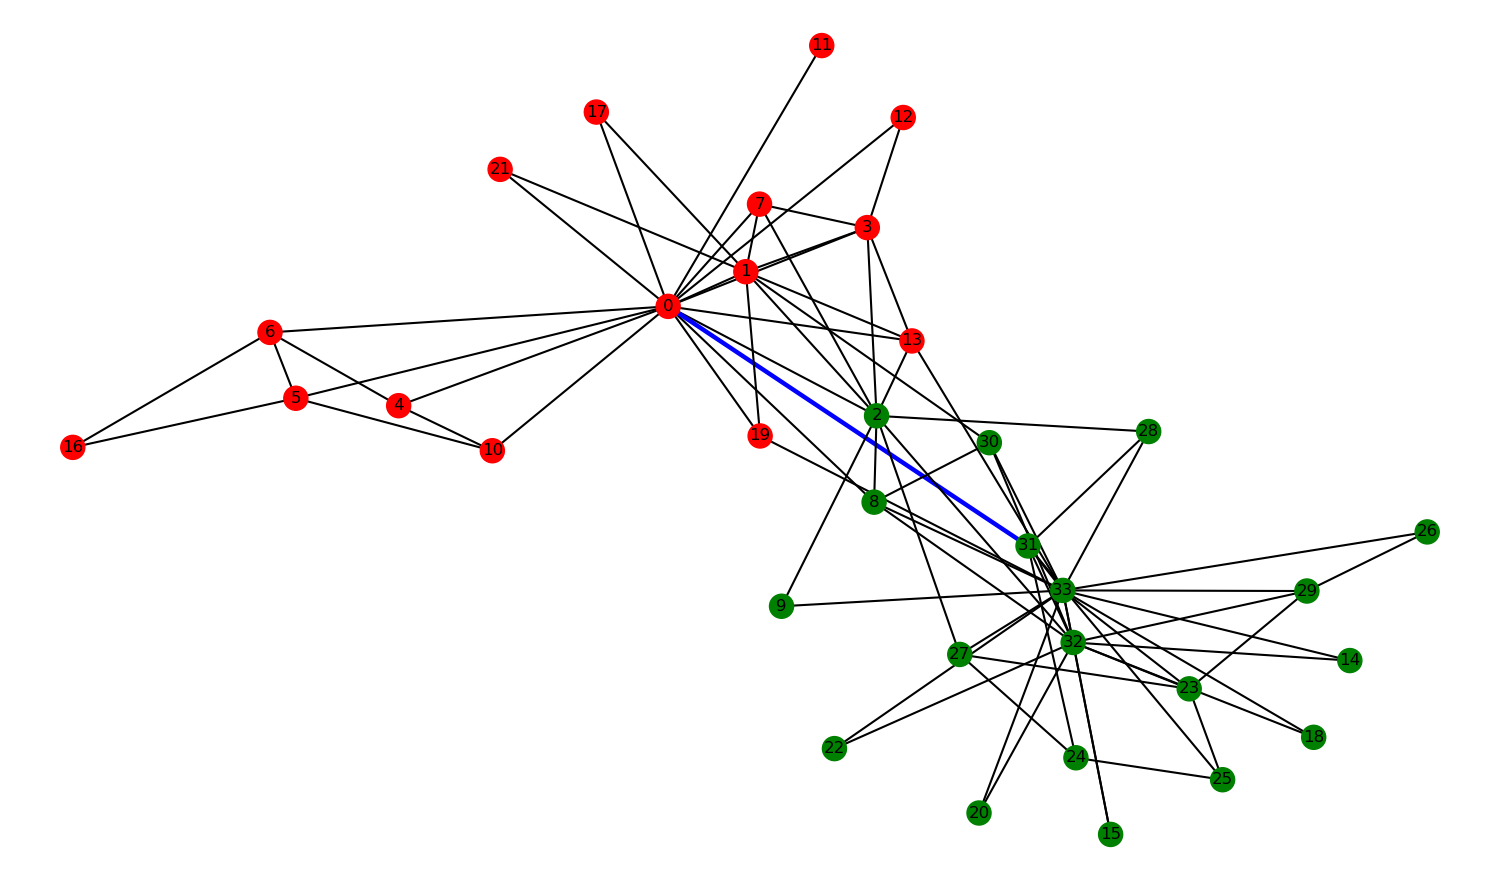
\includegraphics[trim=0 0 0 0, clip, width=127mm] {1x.PNG}
    \caption{Iteration 1 highlighted to remove nodeedge in blue}
    \label{fig:web-growth}
\end{figure}

\begin{figure}[h]
    \centering
    % trim and clip are used to crop the image, trim=left bottom right top
    % width sets max width, height will be scaled appropriately
    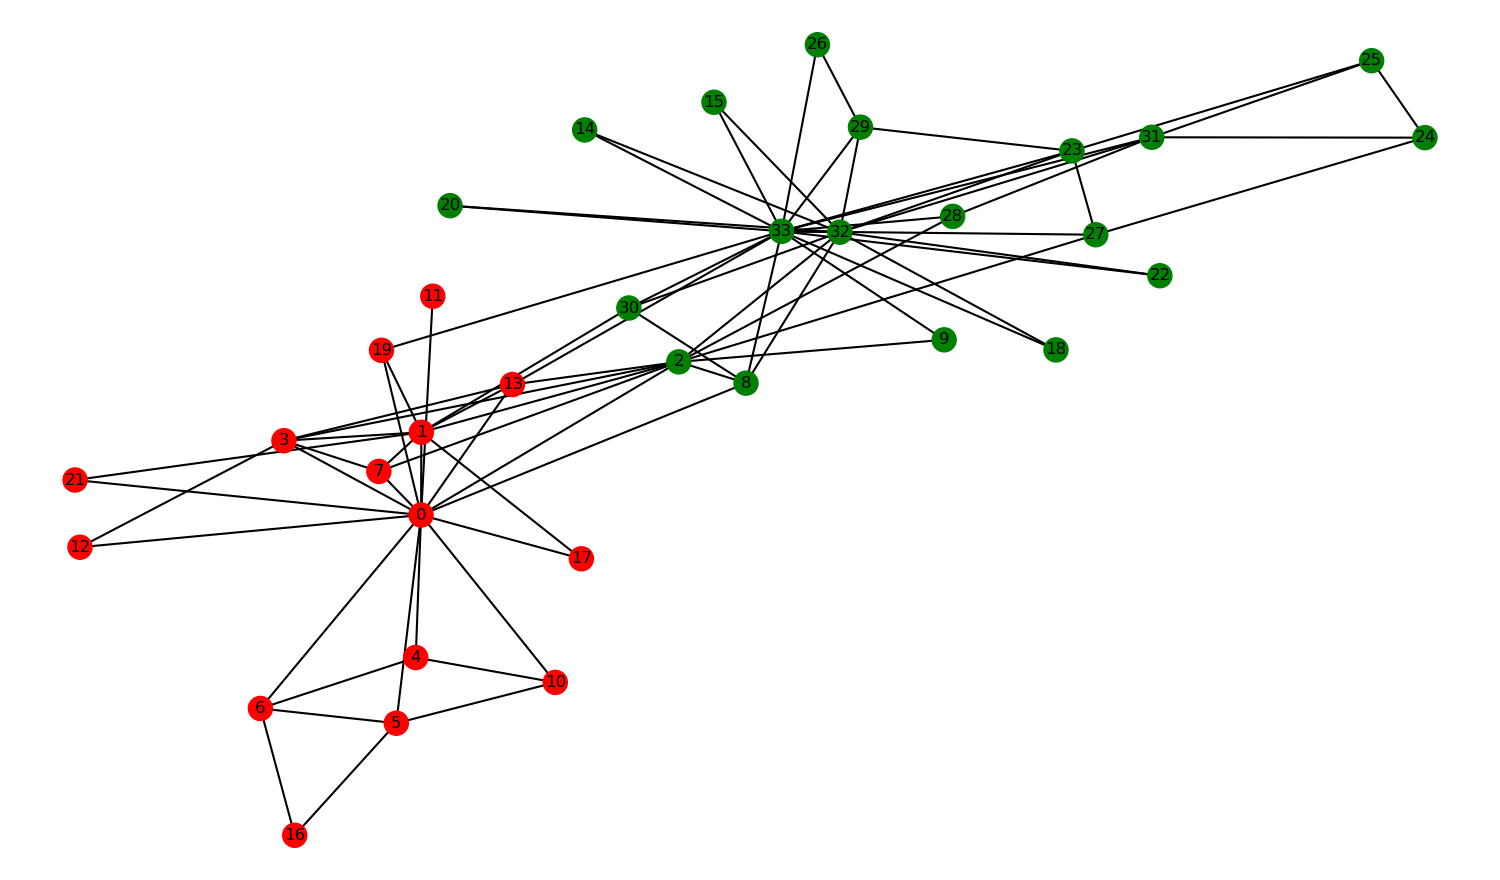
\includegraphics[trim=0 0 0 0, clip, width=127mm] {1y.PNG}
    \caption{Iteration 1 showing nodeedge being removed}
    \label{fig:web-growth}
\end{figure}

\begin{figure}[h]
    \centering
    % trim and clip are used to crop the image, trim=left bottom right top
    % width sets max width, height will be scaled appropriately
    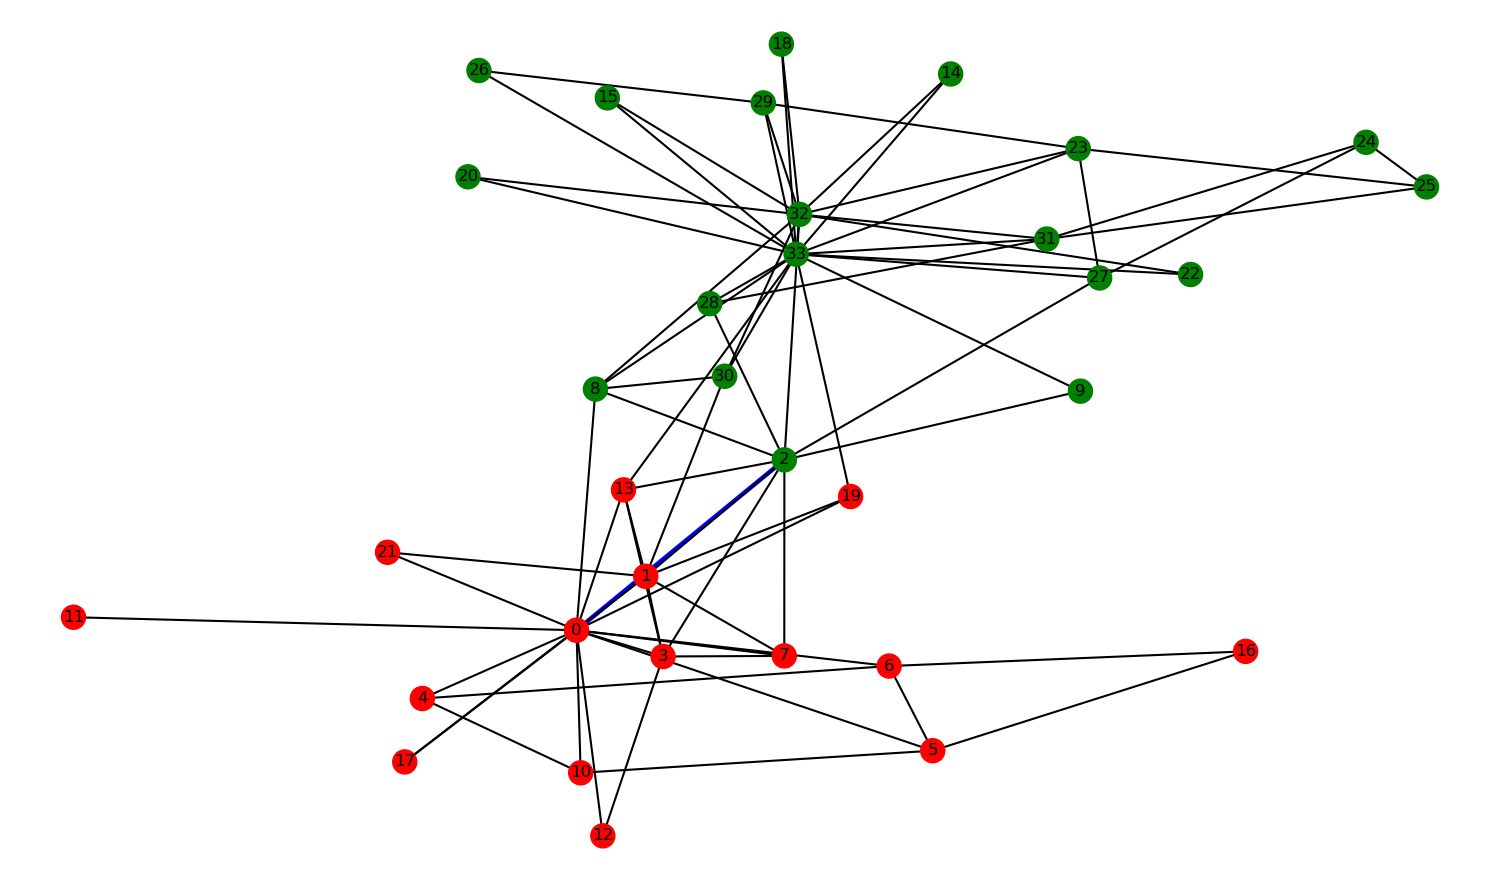
\includegraphics[trim=0 0 0 0, clip, width=127mm] {2x.PNG}
    \caption{Iteration 2 highlighted to remove nodeedge in blue}
    \label{fig:web-growth}
\end{figure}

\begin{figure}[h]
    \centering
    % trim and clip are used to crop the image, trim=left bottom right top
    % width sets max width, height will be scaled appropriately
    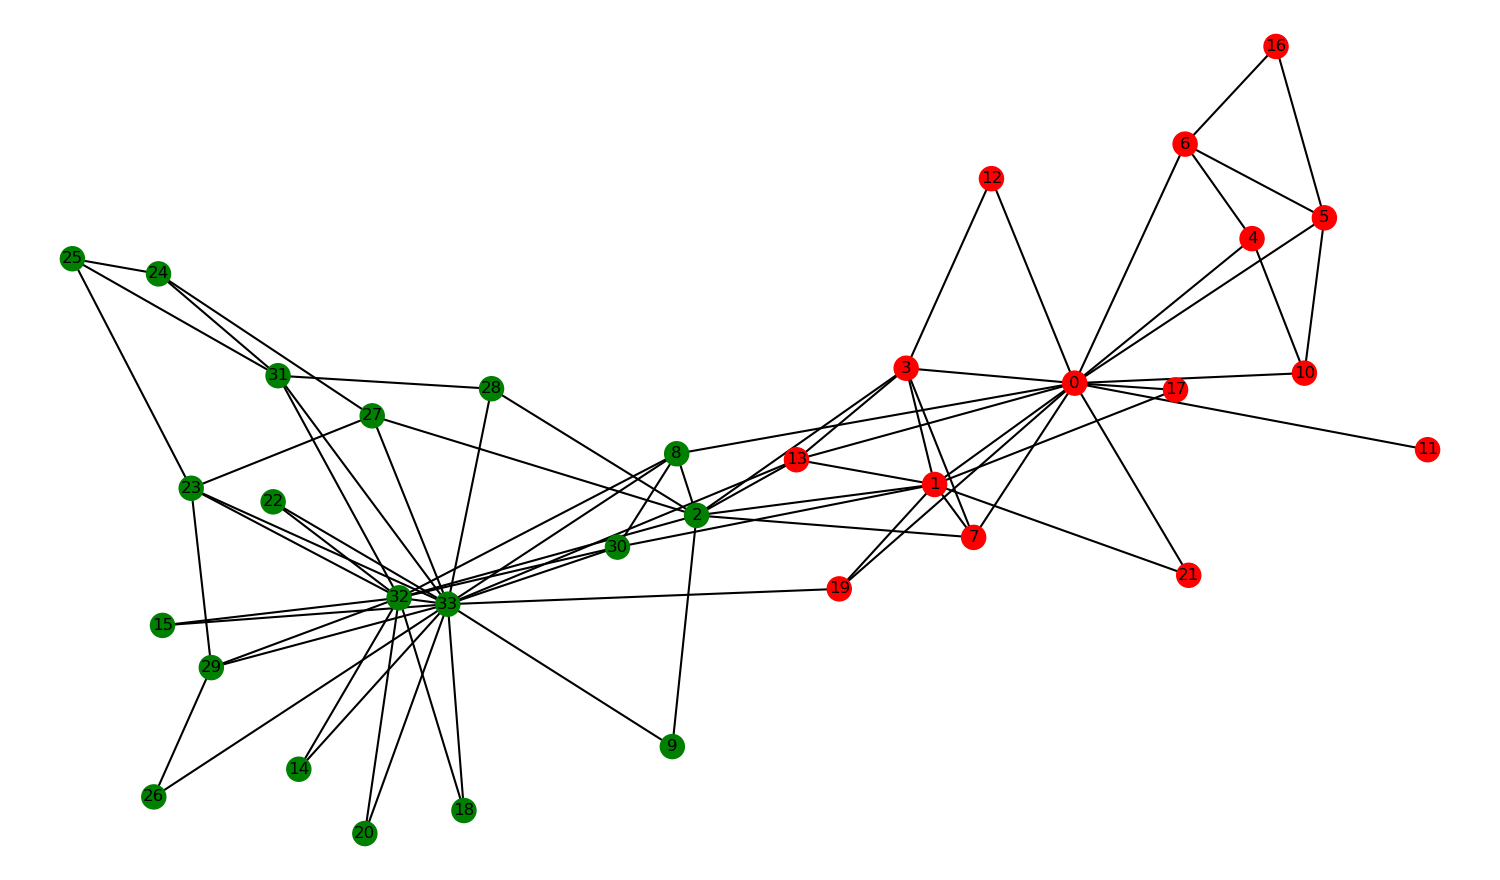
\includegraphics[trim=0 0 0 0, clip, width=127mm] {2y.PNG}
    \caption{Iteration 2 showing nodeedge being removed}
    \label{fig:web-growth}
\end{figure}


\begin{figure}[h]
    \centering
    % trim and clip are used to crop the image, trim=left bottom right top
    % width sets max width, height will be scaled appropriately
    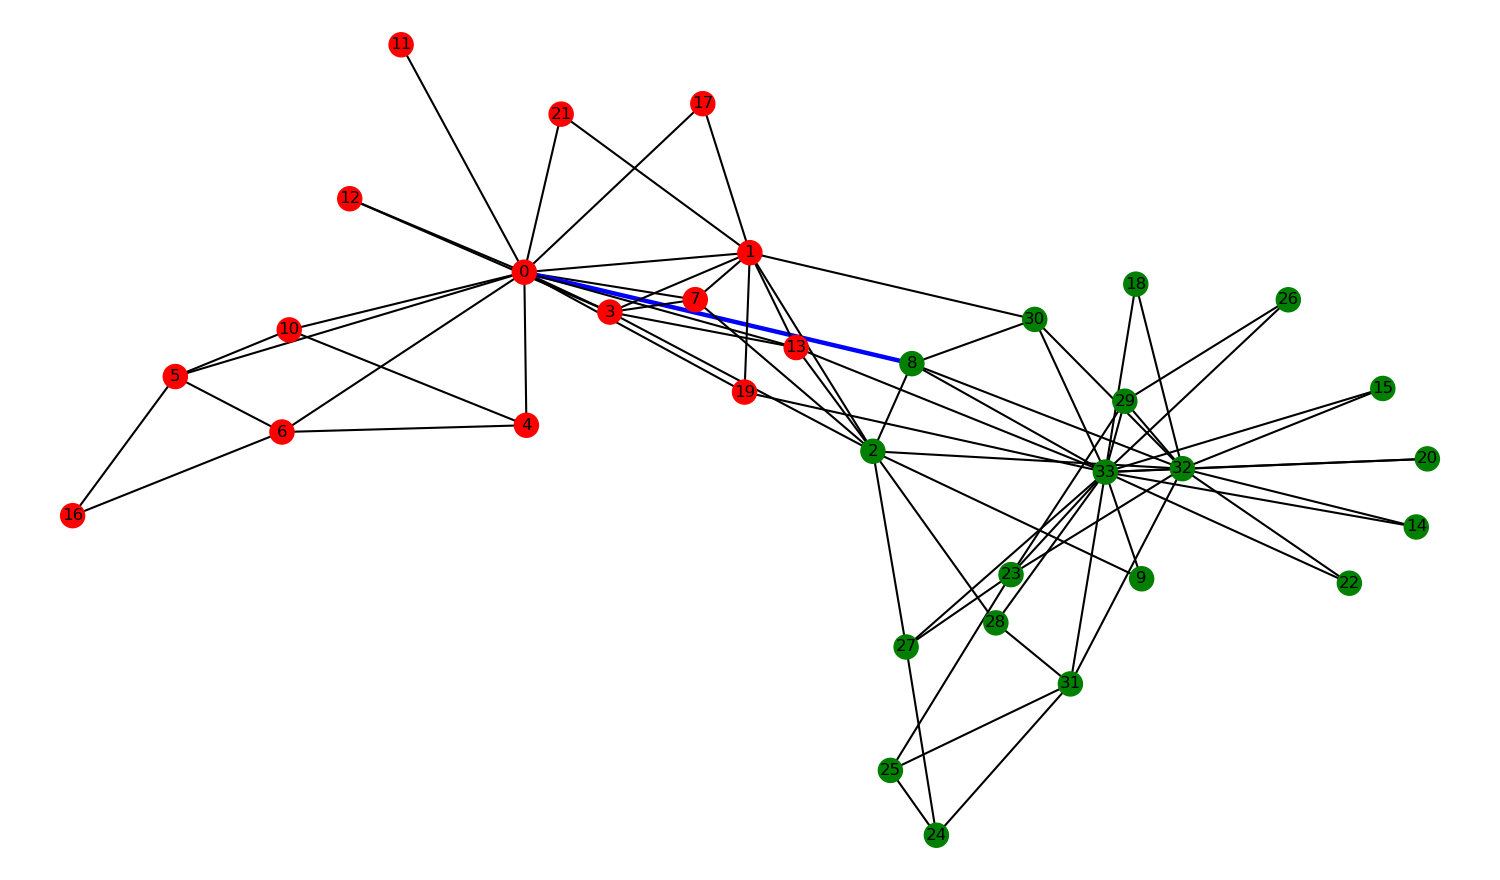
\includegraphics[trim=0 0 0 0, clip, width=127mm] {3x.PNG}
    \caption{Iteration 3 highlighted to remove nodeedge in blue}
    \label{fig:web-growth}
\end{figure}

\begin{figure}[h]
    \centering
    % trim and clip are used to crop the image, trim=left bottom right top
    % width sets max width, height will be scaled appropriately
    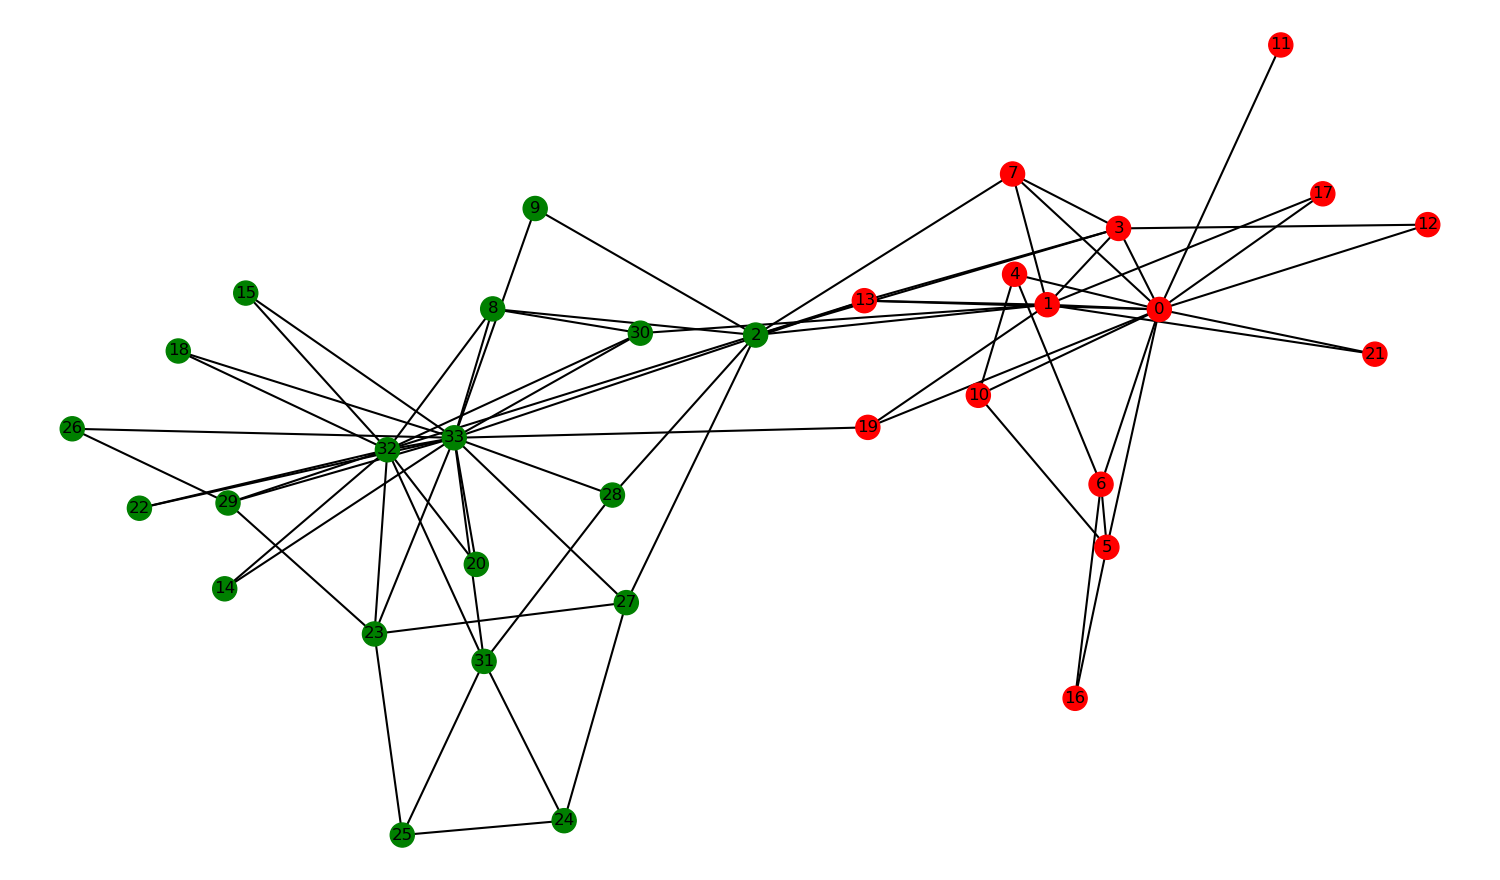
\includegraphics[trim=0 0 0 0, clip, width=127mm] {3y.PNG}
    \caption{Iteration 3 showing nodeedge being removed}
    \label{fig:web-growth}
\end{figure}

\begin{figure}[h]
    \centering
    % trim and clip are used to crop the image, trim=left bottom right top
    % width sets max width, height will be scaled appropriately
    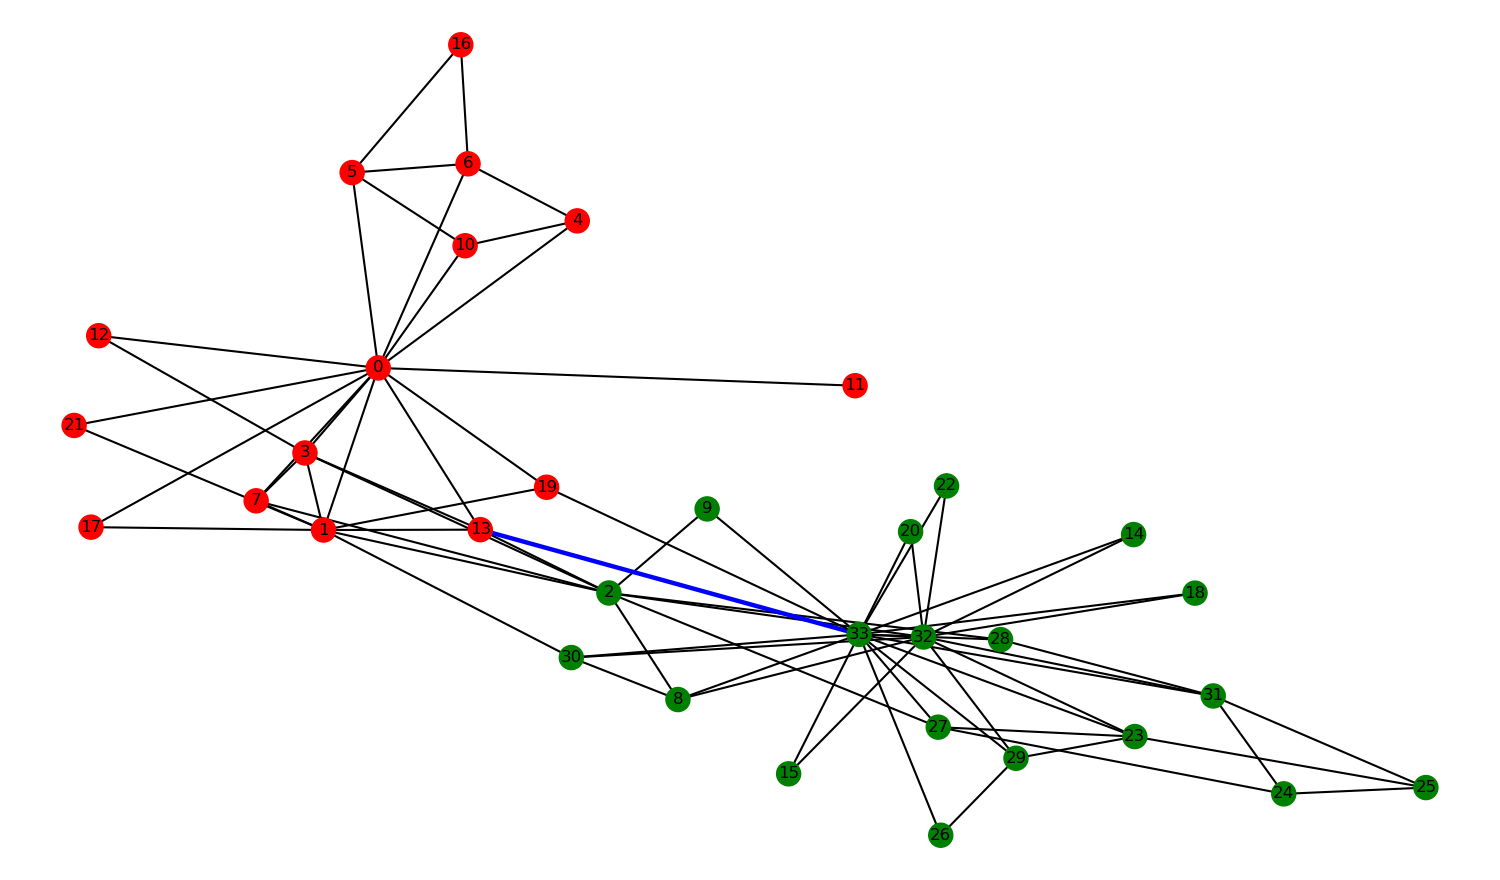
\includegraphics[trim=0 0 0 0, clip, width=127mm] {4x.PNG}
    \caption{Iteration 4 highlighted to remove nodeedge in blue}
    \label{fig:web-growth}
\end{figure}

\begin{figure}[h]
    \centering
    % trim and clip are used to crop the image, trim=left bottom right top
    % width sets max width, height will be scaled appropriately
    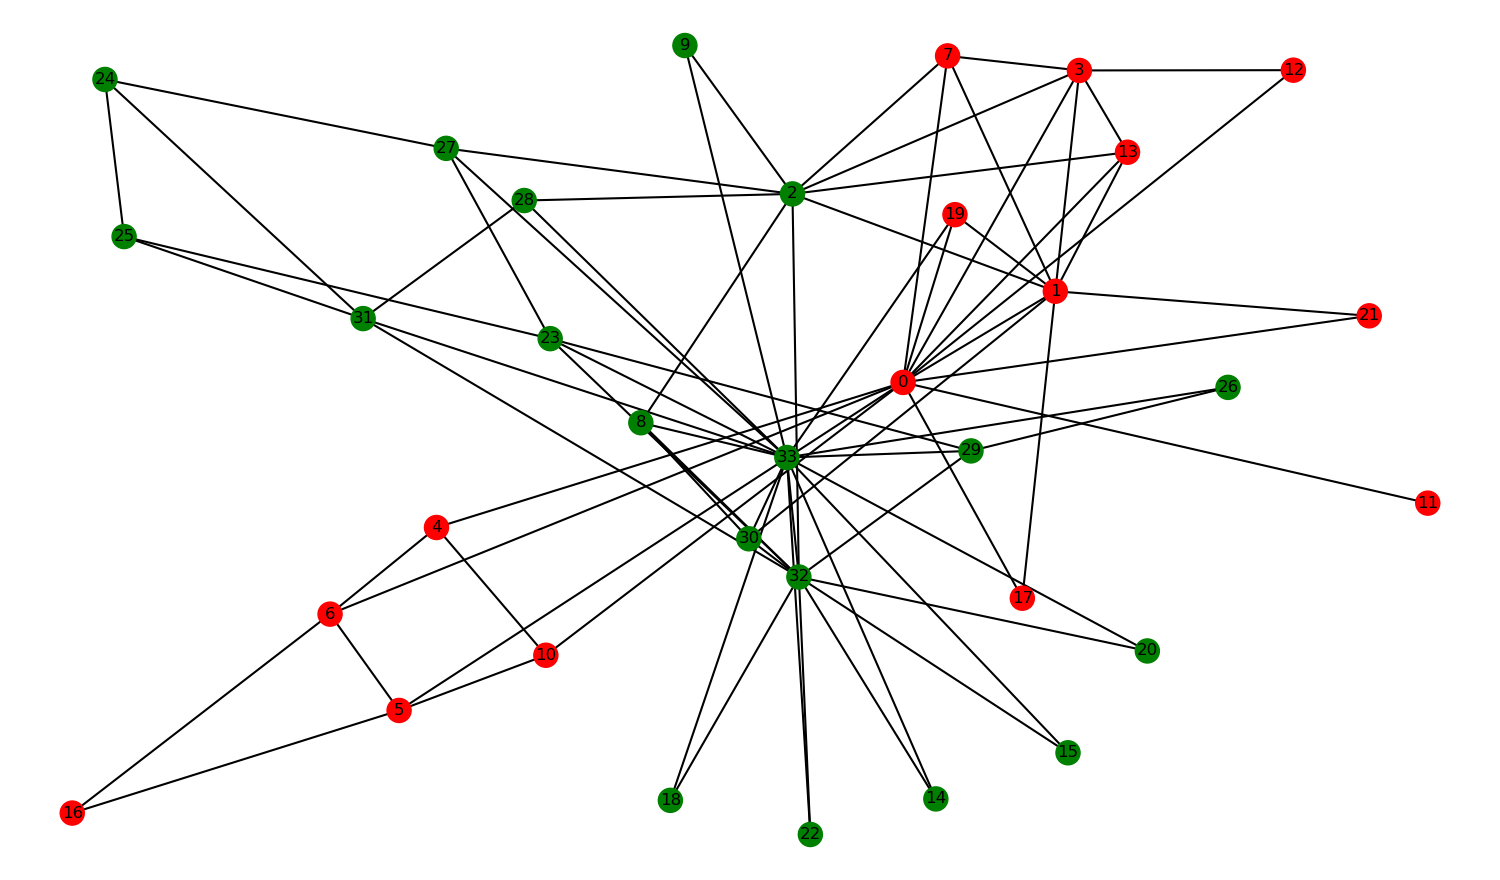
\includegraphics[trim=0 0 0 0, clip, width=127mm] {4y.PNG}
    \caption{Iteration 4 showing nodeedge being removed}
    \label{fig:web-growth}
\end{figure}

\begin{figure}[h]
    \centering
    % trim and clip are used to crop the image, trim=left bottom right top
    % width sets max width, height will be scaled appropriately
    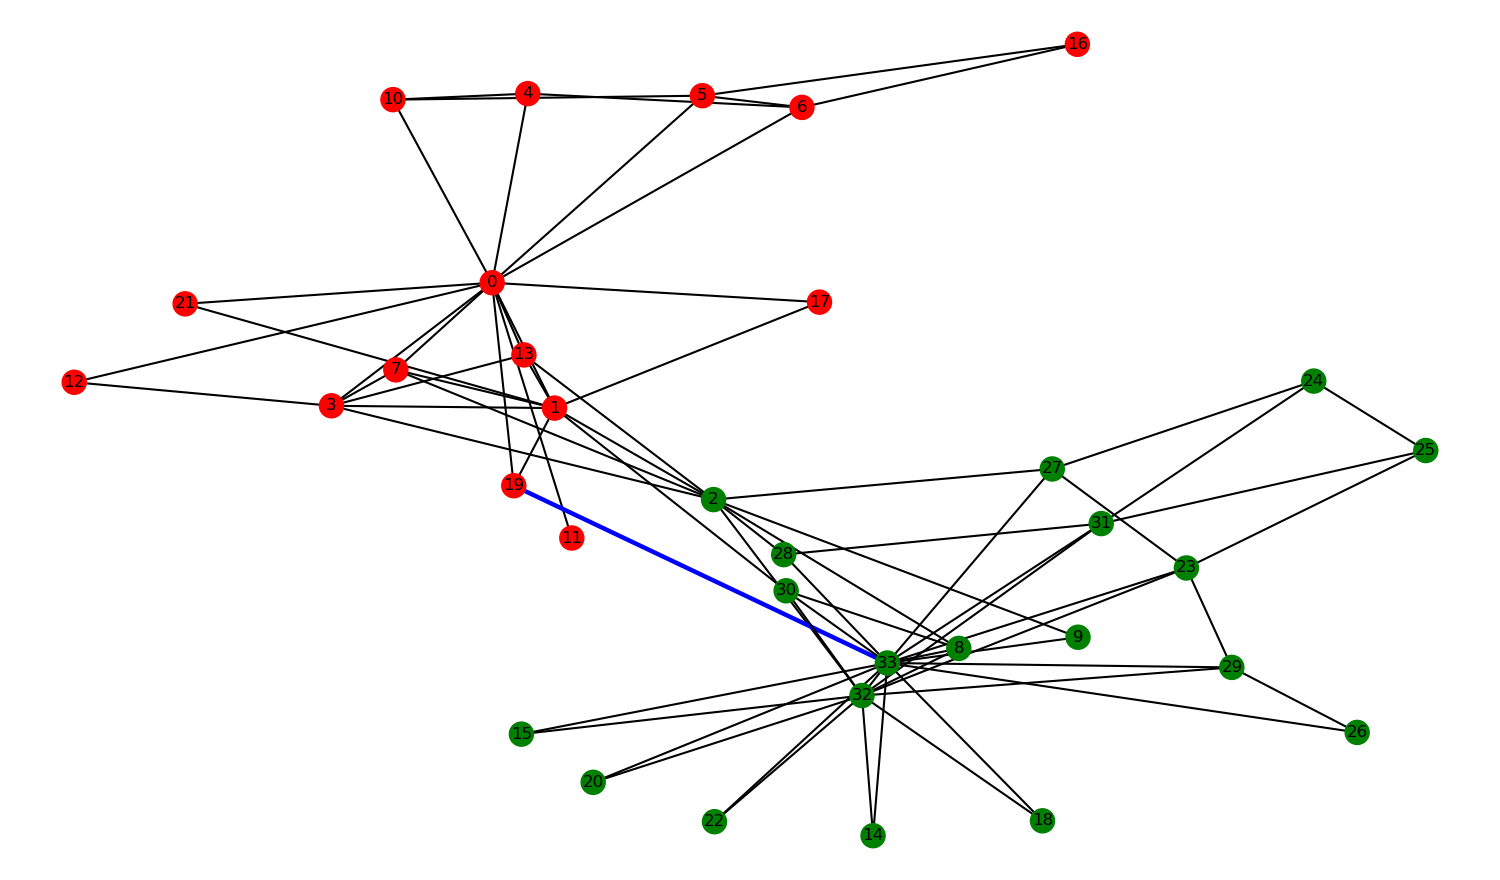
\includegraphics[trim=0 0 0 0, clip, width=127mm] {5x.PNG}
    \caption{Iteration 5 highlighted to remove nodeedge in blue}
    \label{fig:web-growth}
\end{figure}

\begin{figure}[h]
    \centering
    % trim and clip are used to crop the image, trim=left bottom right top
    % width sets max width, height will be scaled appropriately
    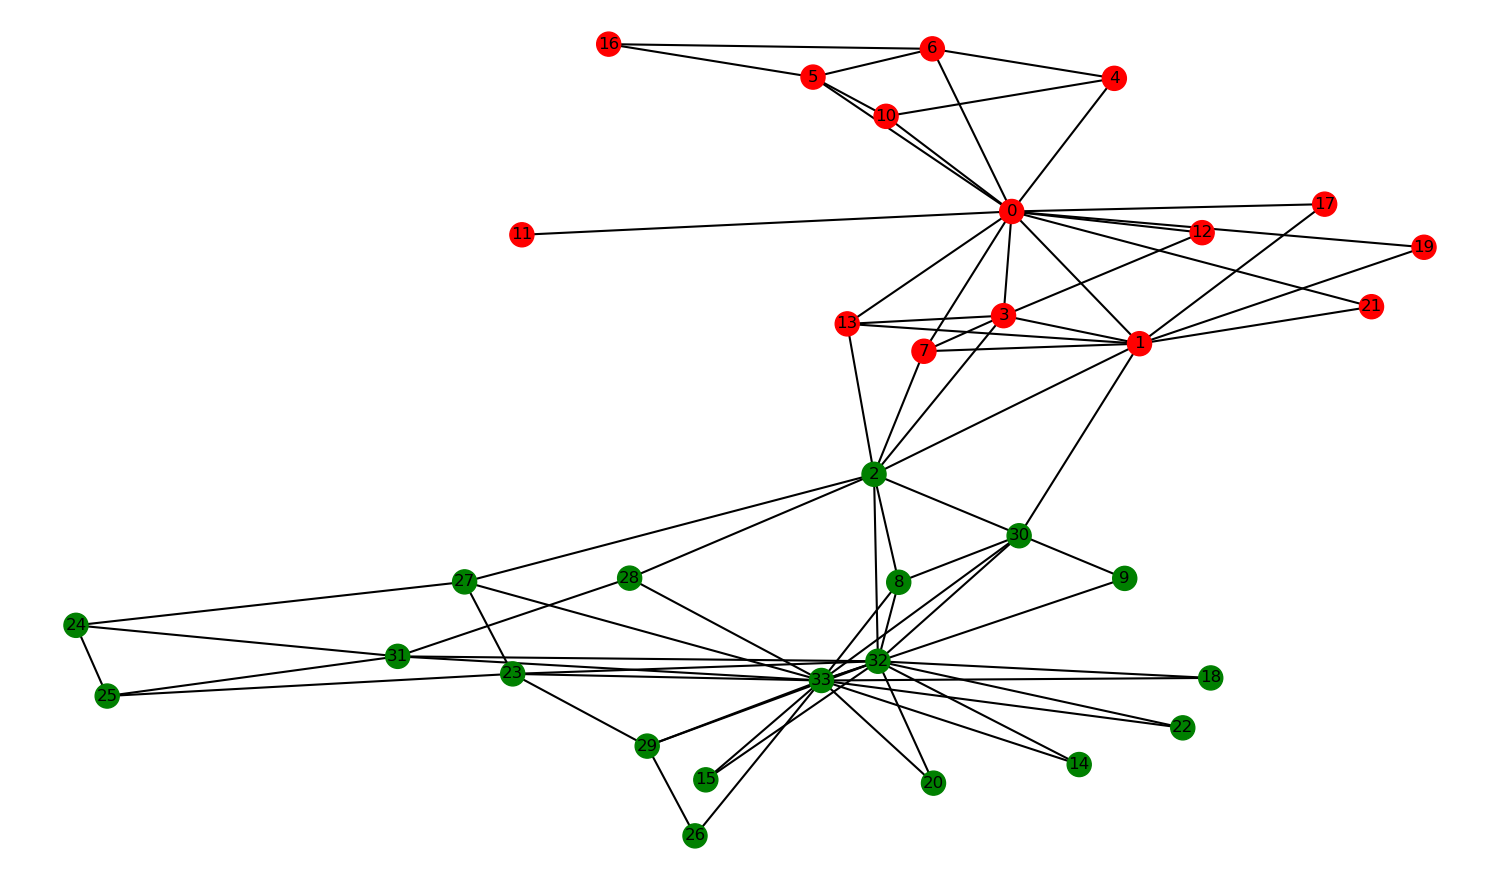
\includegraphics[trim=0 0 0 0, clip, width=127mm] {5y.PNG}
    \caption{Iteration 5 showing nodeedge being removed}
    \label{fig:web-growth}
\end{figure}

\begin{figure}[h]
    \centering
    % trim and clip are used to crop the image, trim=left bottom right top
    % width sets max width, height will be scaled appropriately
    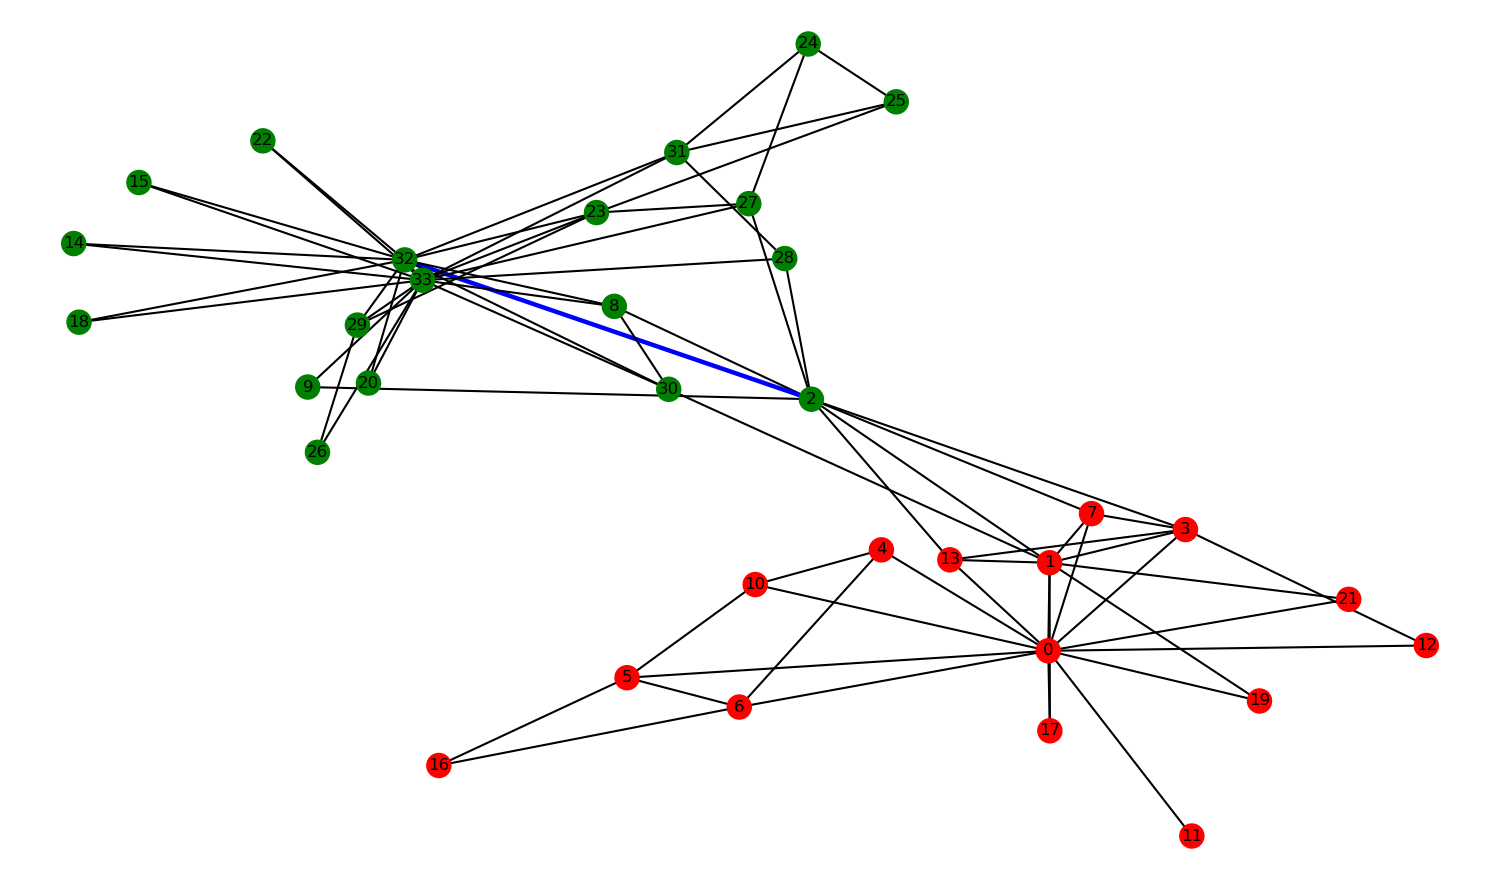
\includegraphics[trim=0 0 0 0, clip, width=127mm] {6x.PNG}
    \caption{Iteration 6 highlighted to remove nodeedge in blue}
    \label{fig:web-growth}
\end{figure}

\begin{figure}[h]
    \centering
    % trim and clip are used to crop the image, trim=left bottom right top
    % width sets max width, height will be scaled appropriately
    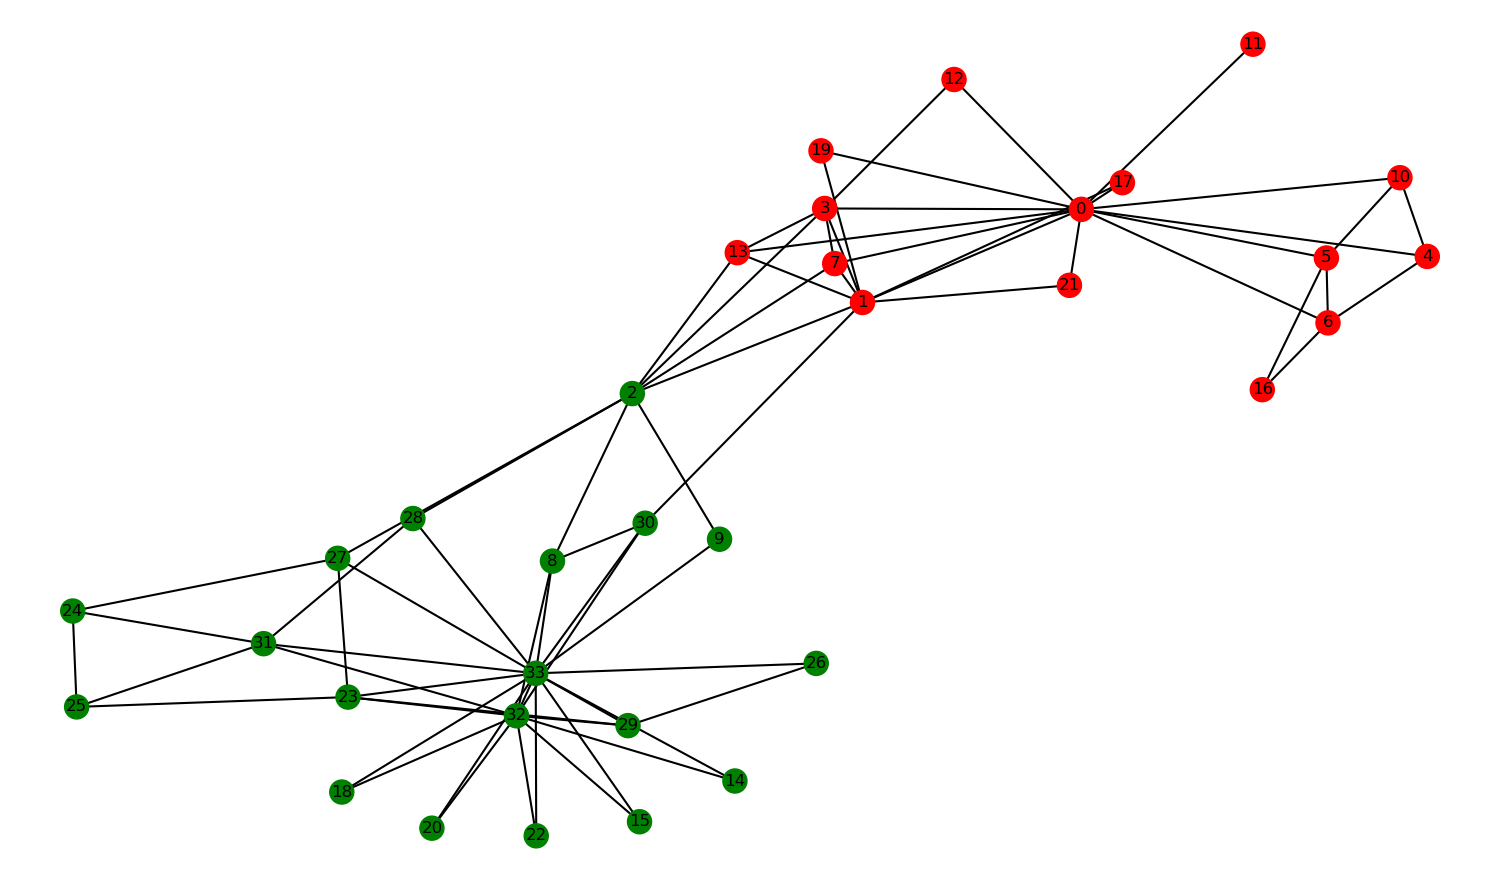
\includegraphics[trim=0 0 0 0, clip, width=127mm] {6y.PNG}
    \caption{Iteration 6 showing nodeedge being removed}
    \label{fig:web-growth}
\end{figure}

\begin{figure}[h]
    \centering
    % trim and clip are used to crop the image, trim=left bottom right top
    % width sets max width, height will be scaled appropriately
    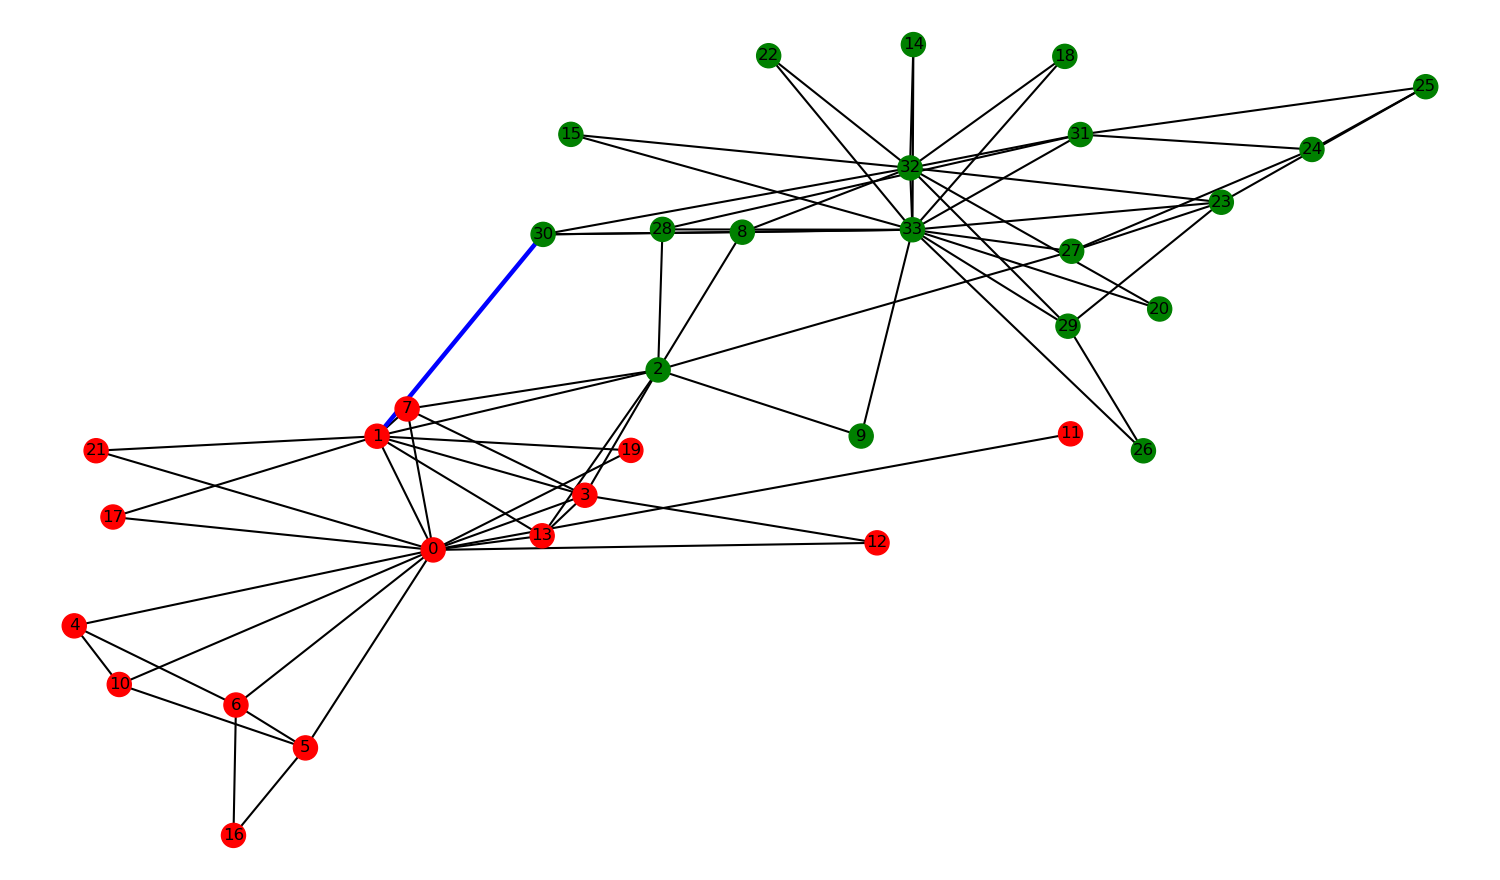
\includegraphics[trim=0 0 0 0, clip, width=127mm] {7x.PNG}
    \caption{Iteration 7 highlighted to remove nodeedge in blue}
    \label{fig:web-growth}
\end{figure}

\begin{figure}[h]
    \centering
    % trim and clip are used to crop the image, trim=left bottom right top
    % width sets max width, height will be scaled appropriately
    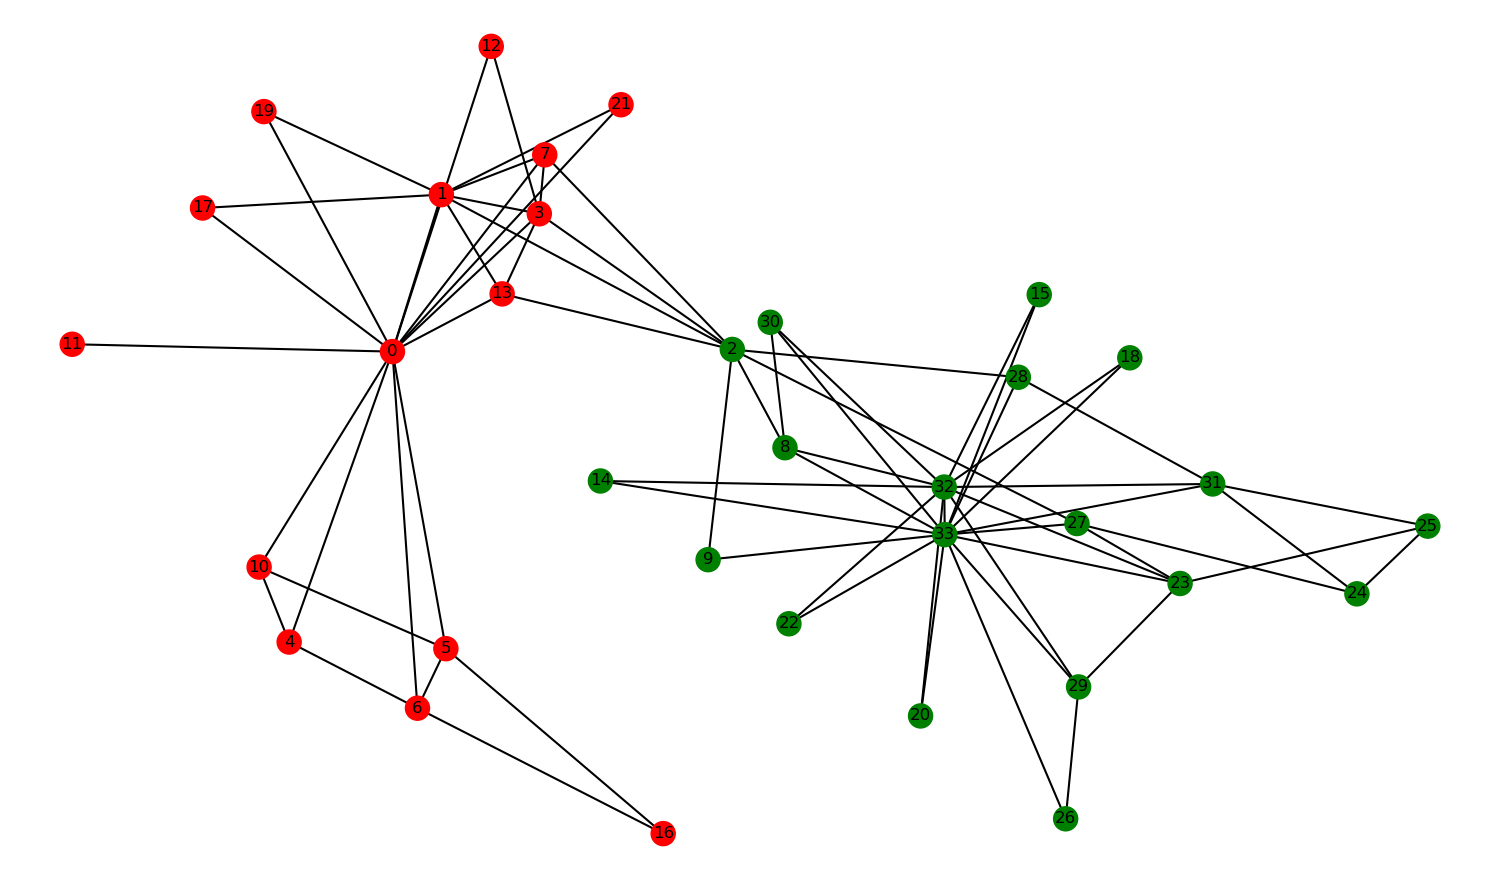
\includegraphics[trim=0 0 0 0, clip, width=127mm] {7y.PNG}
    \caption{Iteration 7 showing nodeedge being removed}
    \label{fig:web-growth}
\end{figure}

\begin{figure}[h]
    \centering
    % trim and clip are used to crop the image, trim=left bottom right top
    % width sets max width, height will be scaled appropriately
    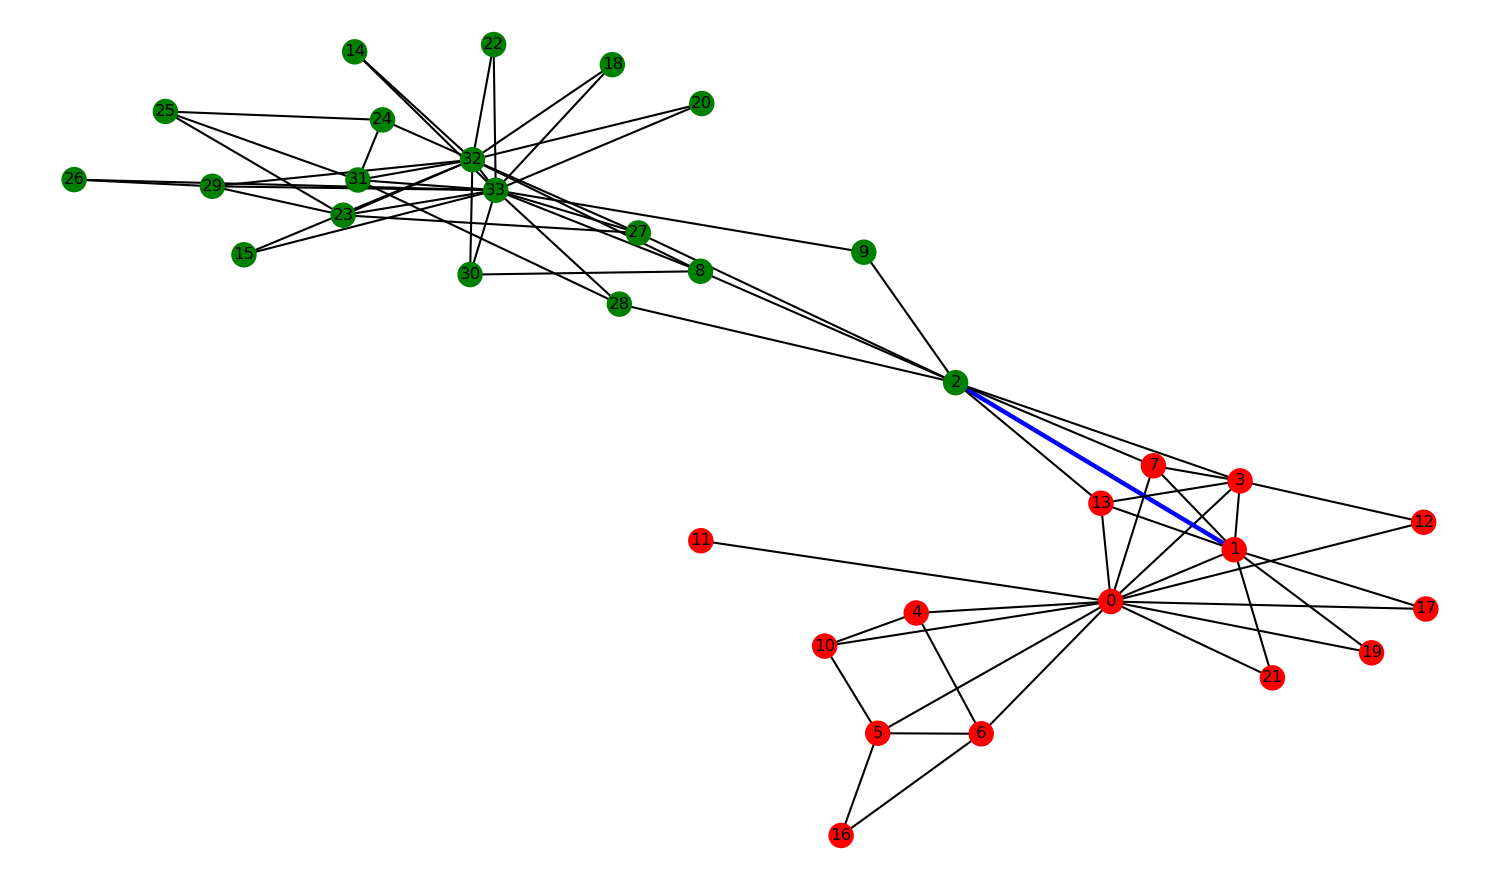
\includegraphics[trim=0 0 0 0, clip, width=127mm] {8x.PNG}
    \caption{Iteration 8 highlighted to remove nodeedge in blue}
    \label{fig:web-growth}
\end{figure}

\begin{figure}[h]
    \centering
    % trim and clip are used to crop the image, trim=left bottom right top
    % width sets max width, height will be scaled appropriately
    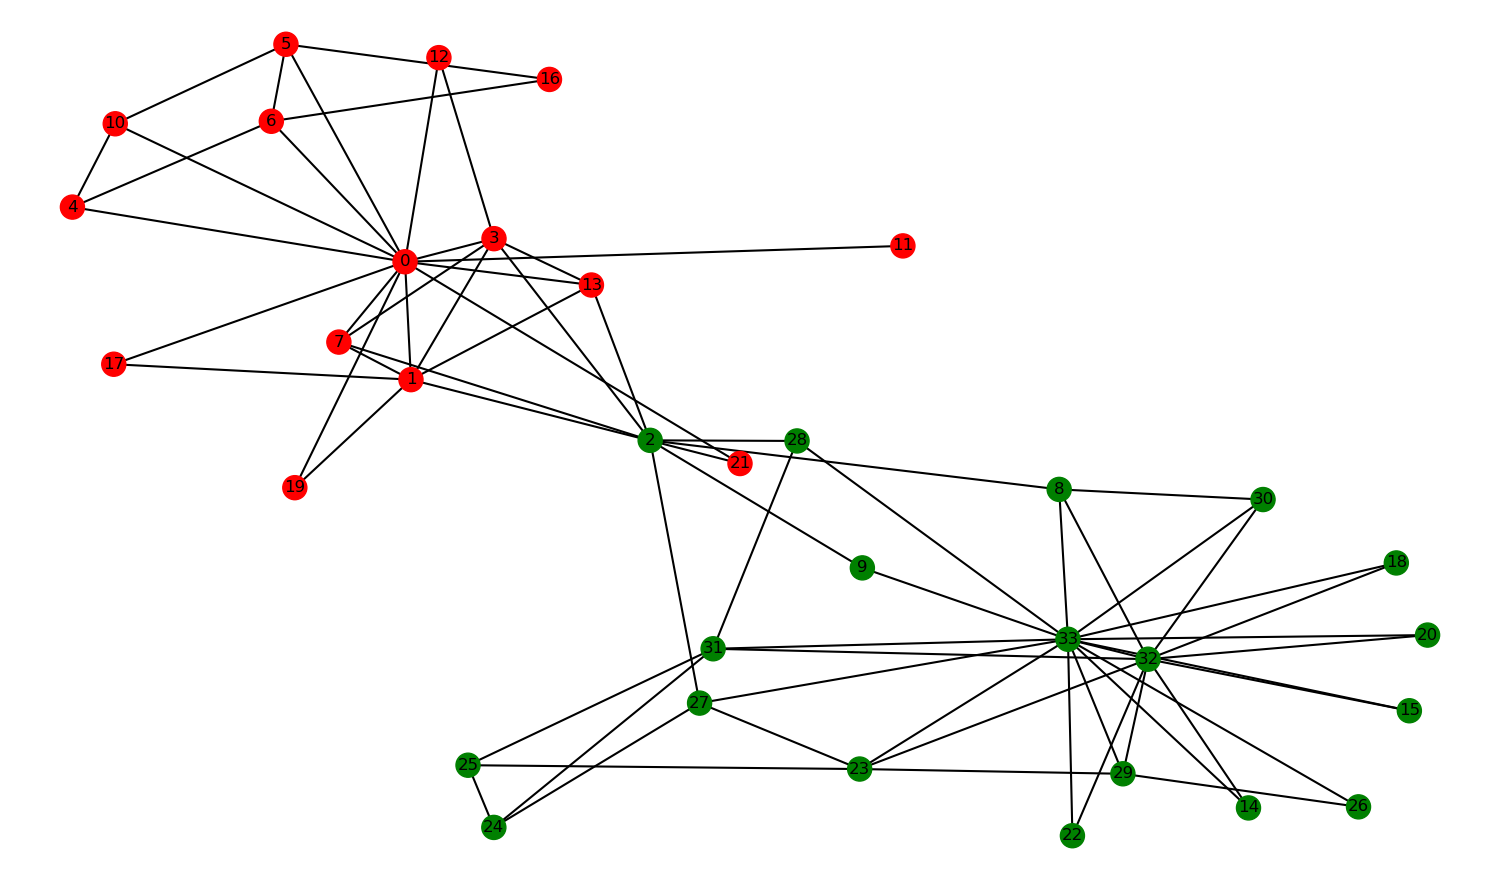
\includegraphics[trim=0 0 0 0, clip, width=127mm] {8y.PNG}
    \caption{Iteration 8 showing nodeedge being removed}
    \label{fig:web-growth}
\end{figure}

\begin{figure}[h]
    \centering
    % trim and clip are used to crop the image, trim=left bottom right top
    % width sets max width, height will be scaled appropriately
    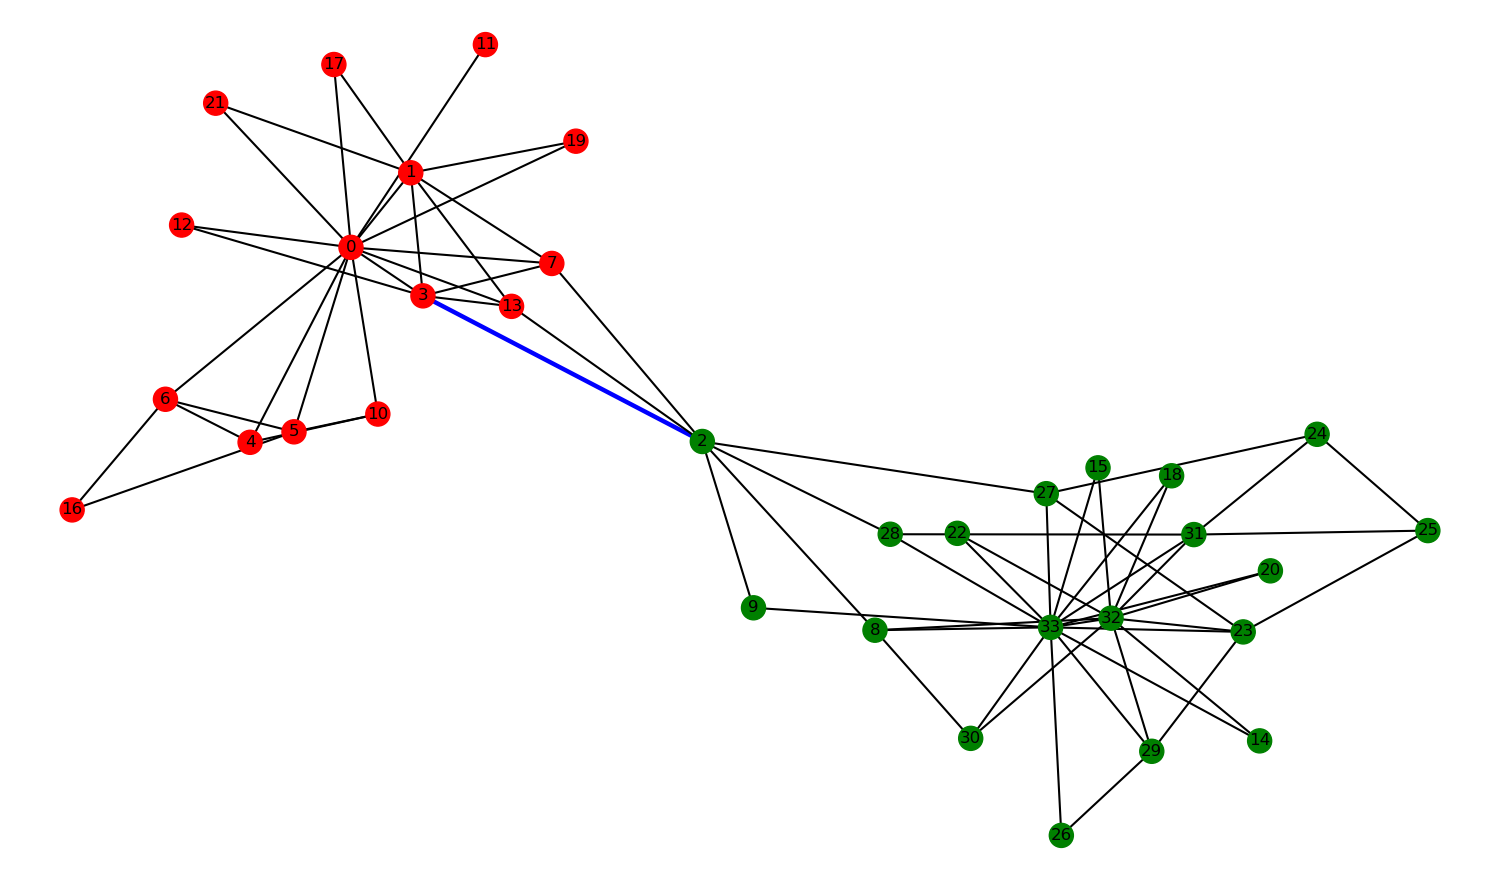
\includegraphics[trim=0 0 0 0, clip, width=127mm] {9x.PNG}
    \caption{Iteration 9 highlighted to remove nodeedge in blue}
    \label{fig:web-growth}
\end{figure}

\begin{figure}[h]
    \centering
    % trim and clip are used to crop the image, trim=left bottom right top
    % width sets max width, height will be scaled appropriately
    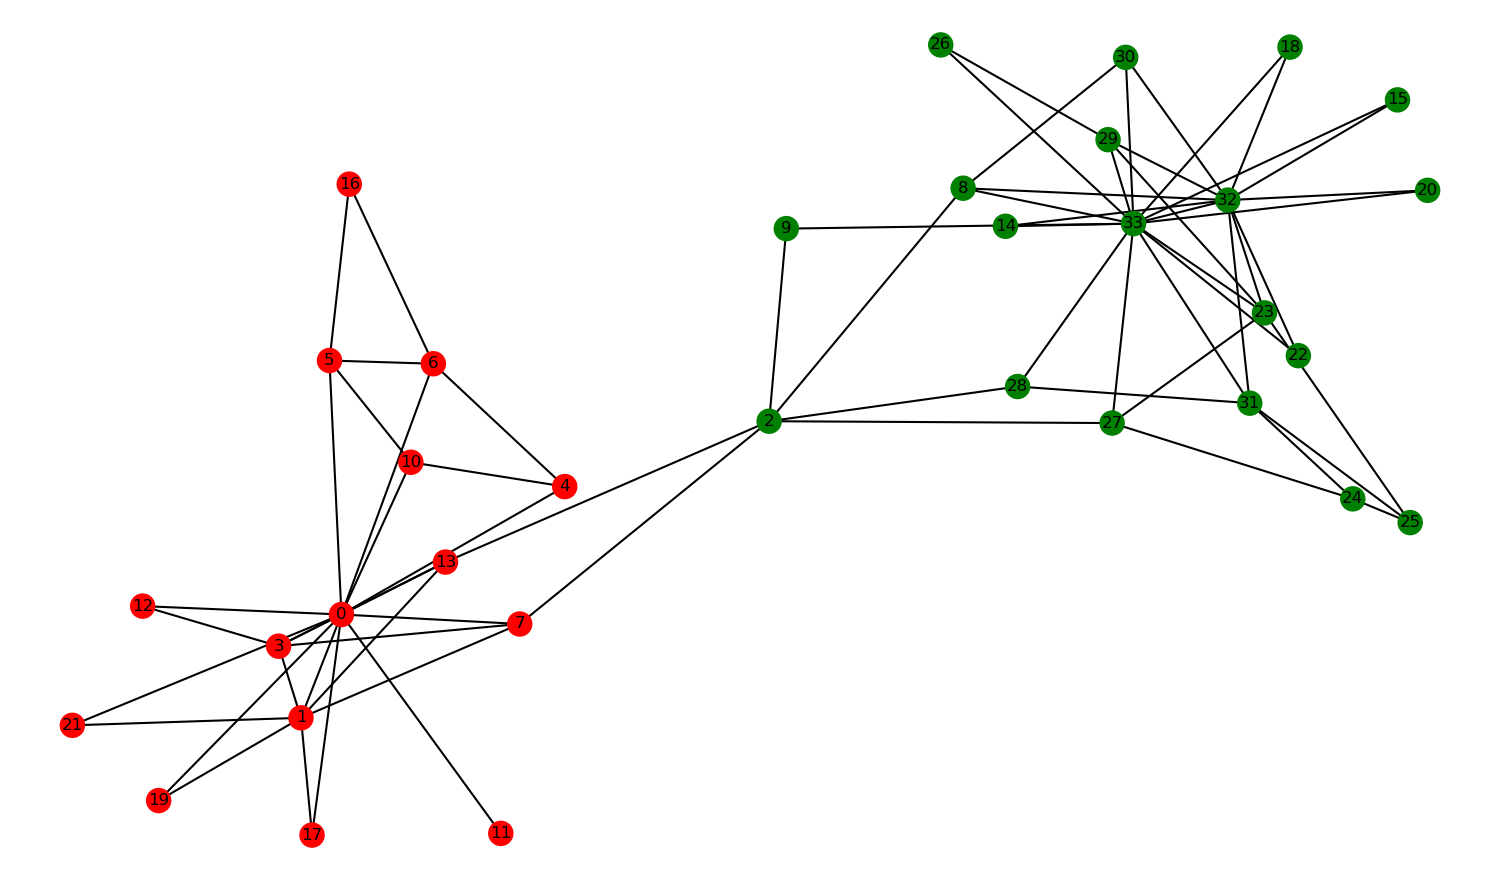
\includegraphics[trim=0 0 0 0, clip, width=127mm] {9y.PNG}
    \caption{Iteration 9 showing nodeedge being removed}
    \label{fig:web-growth}
\end{figure}

\begin{figure}[h]
    \centering
    % trim and clip are used to crop the image, trim=left bottom right top
    % width sets max width, height will be scaled appropriately
    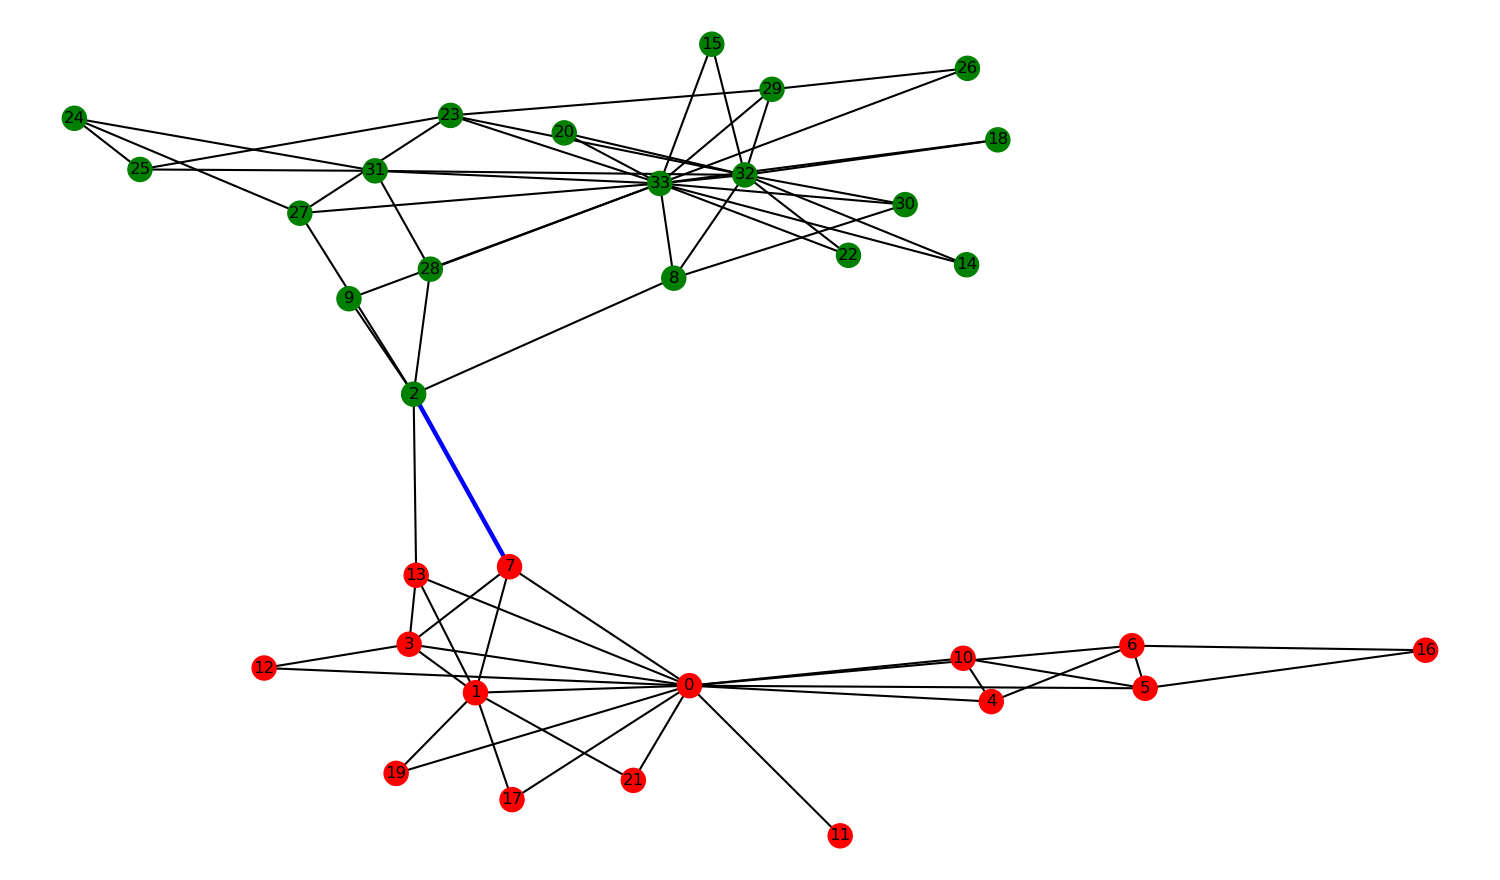
\includegraphics[trim=0 0 0 0, clip, width=127mm] {10x.PNG}
    \caption{Iteration 10 highlighted to remove nodeedge in blue}
    \label{fig:web-growth}
\end{figure}

\begin{figure}[h]
    \centering
    % trim and clip are used to crop the image, trim=left bottom right top
    % width sets max width, height will be scaled appropriately
    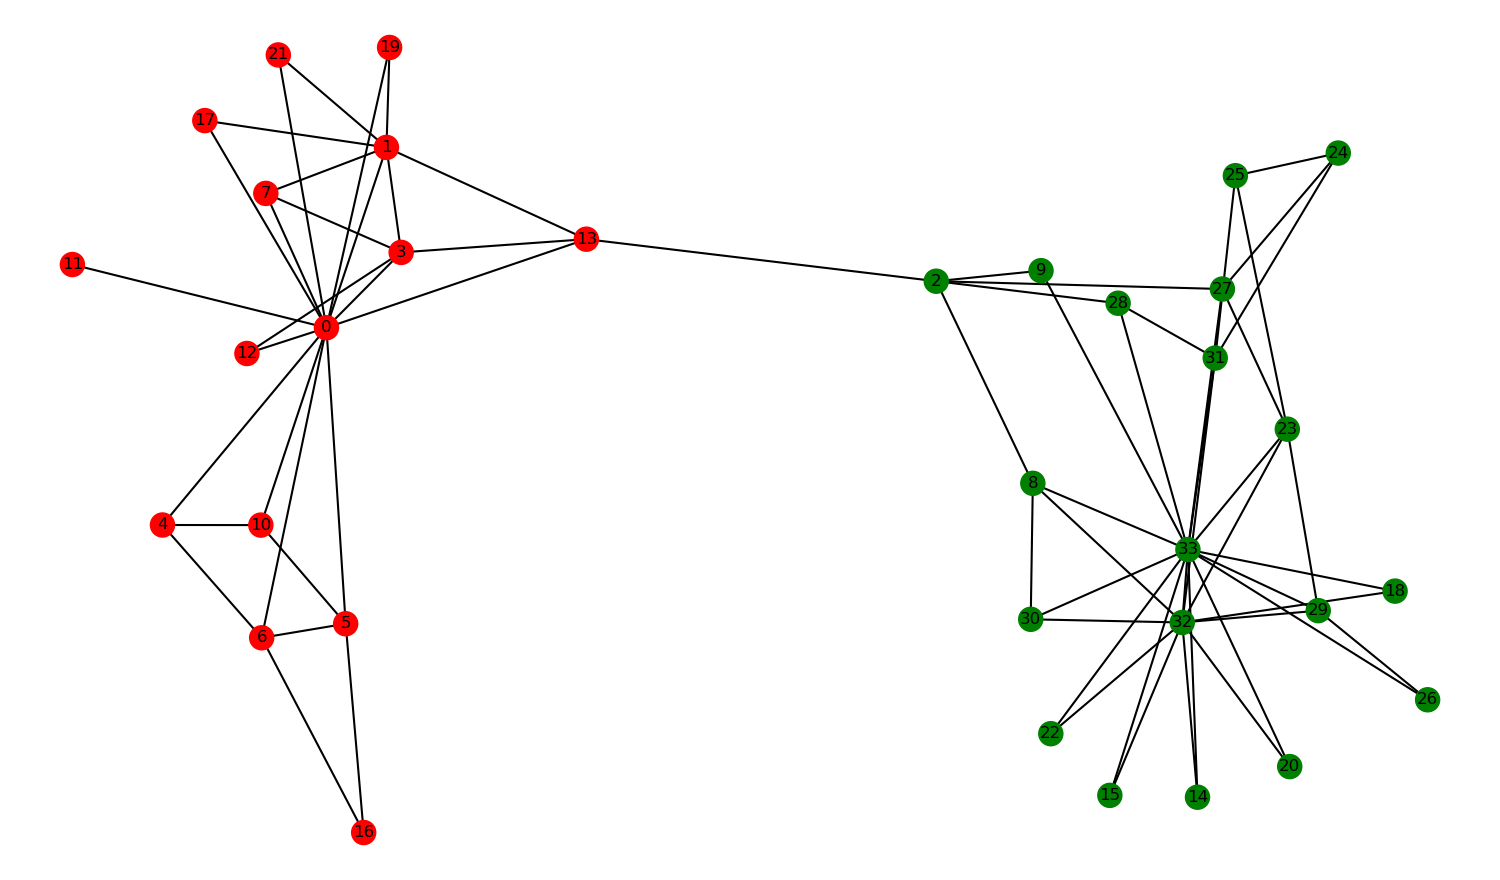
\includegraphics[trim=0 0 0 0, clip, width=127mm] {10y.PNG}
    \caption{Iteration 10 showing nodeedge being removed}
    \label{fig:web-growth}
\end{figure}

\begin{figure}[h]
    \centering
    % trim and clip are used to crop the image, trim=left bottom right top
    % width sets max width, height will be scaled appropriately
    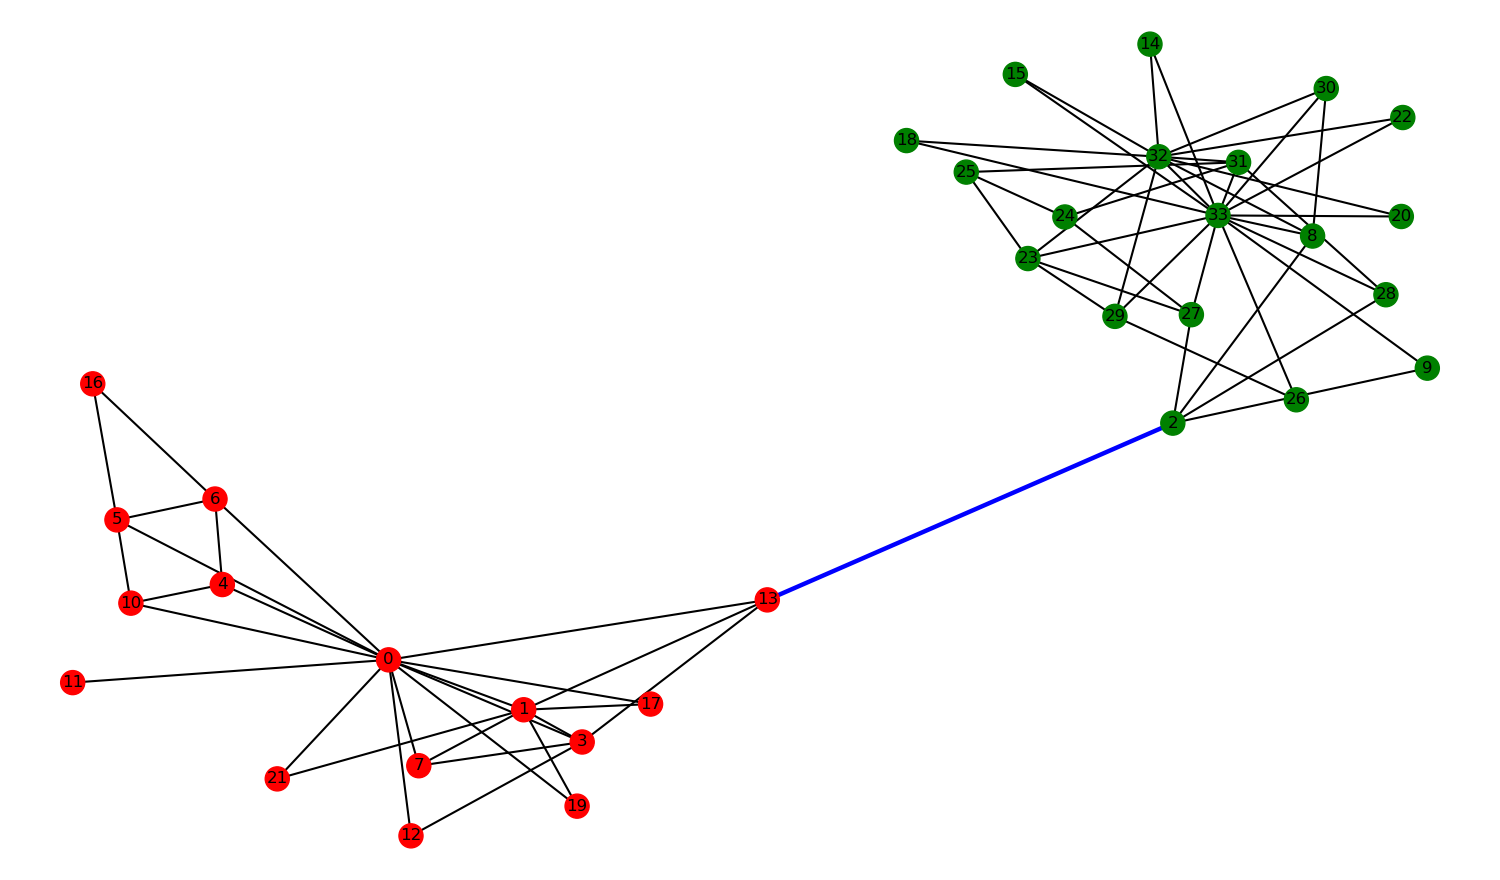
\includegraphics[trim=0 0 0 0, clip, width=127mm] {11x.PNG}
    \caption{Iteration 11 highlighted to remove nodeedge in blue}
    \label{fig:web-growth}
\end{figure}

\begin{figure}[h]
    \centering
    % trim and clip are used to crop the image, trim=left bottom right top
    % width sets max width, height will be scaled appropriately
    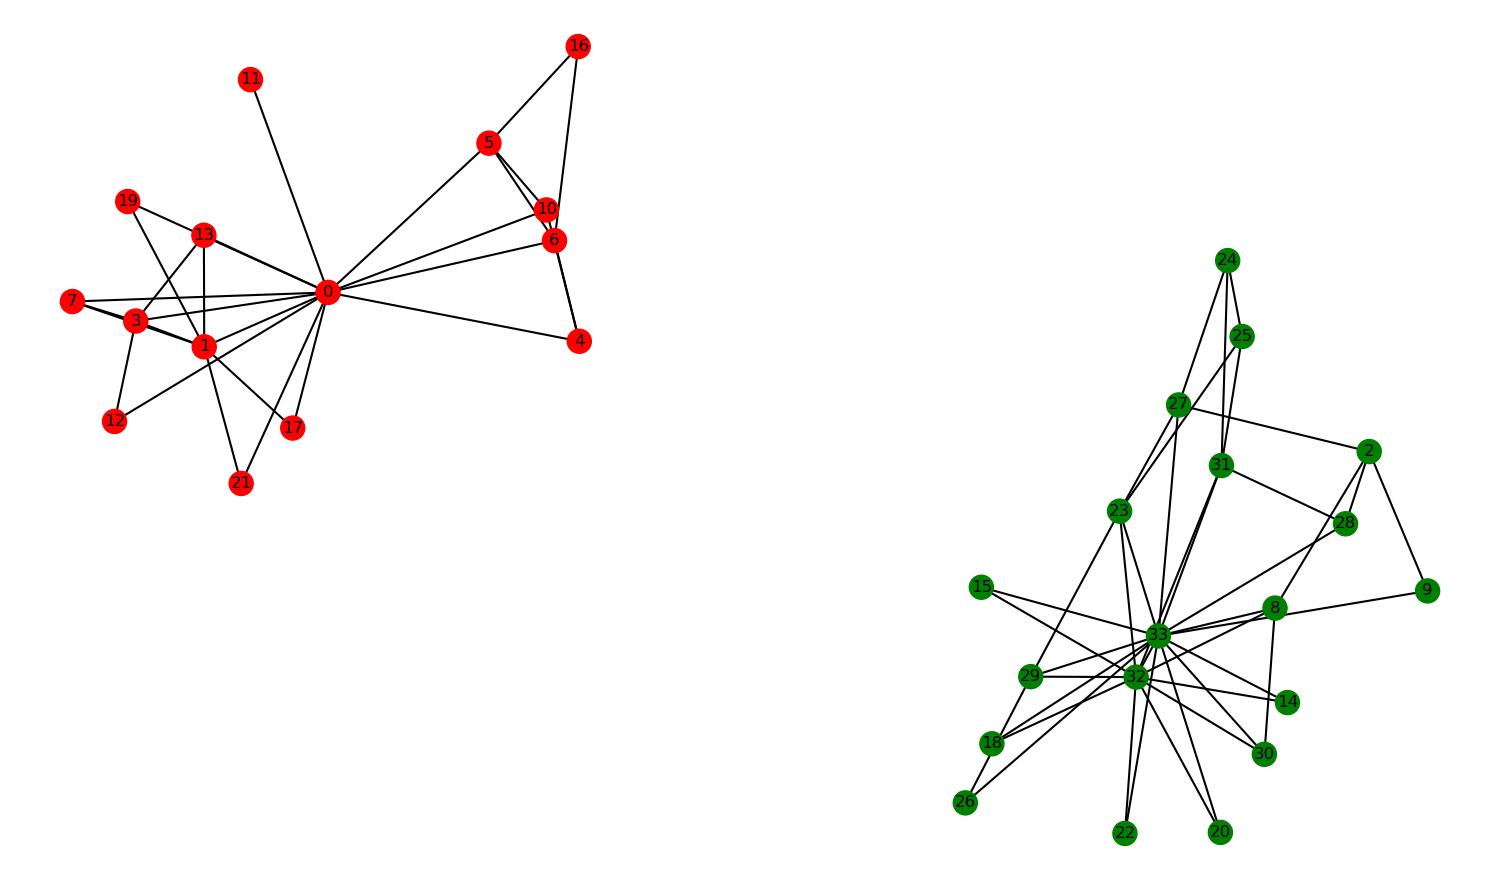
\includegraphics[trim=0 0 0 0, clip, width=127mm] {11y.PNG}
    \caption{Iteration 11 showing nodeedge being removed}
    \label{fig:web-growth}
\end{figure}

\clearpage
\subsection*{Discussion}
In the girvannewman\_graph() the edge betweenness is calculated for each edge in the graph i.e., it finds the best edge and it is returned as a list is stored in bestedge. Then, it removes the edge with highest betweenness. The betweenness is calculated for all the other nodes and they are reset back with the weights. The edge betweenness returns a dictionary, which is then made to a list, sorted and returns the edge with highest betweenness. The coloredges() builds the edge color list and width of the edge list, to set the color coding and the width variable. 


\emph{Q: How many iterations did it take to split the graph?}

Iterations of the Girvan-Newman graph partioning algorithm is run and it took 11 iteration to complete break the graph into two. 

\section*{Q3}
Compare the connected components of the Girvan-Newman split graph (Q2) with the connected components of the actual split Karate club graph (Q1).

\subsection*{Answer}
\begin{figure}[h]
    \centering
    % trim and clip are used to crop the image, trim=left bottom right top
    % width sets max width, height will be scaled appropriately
    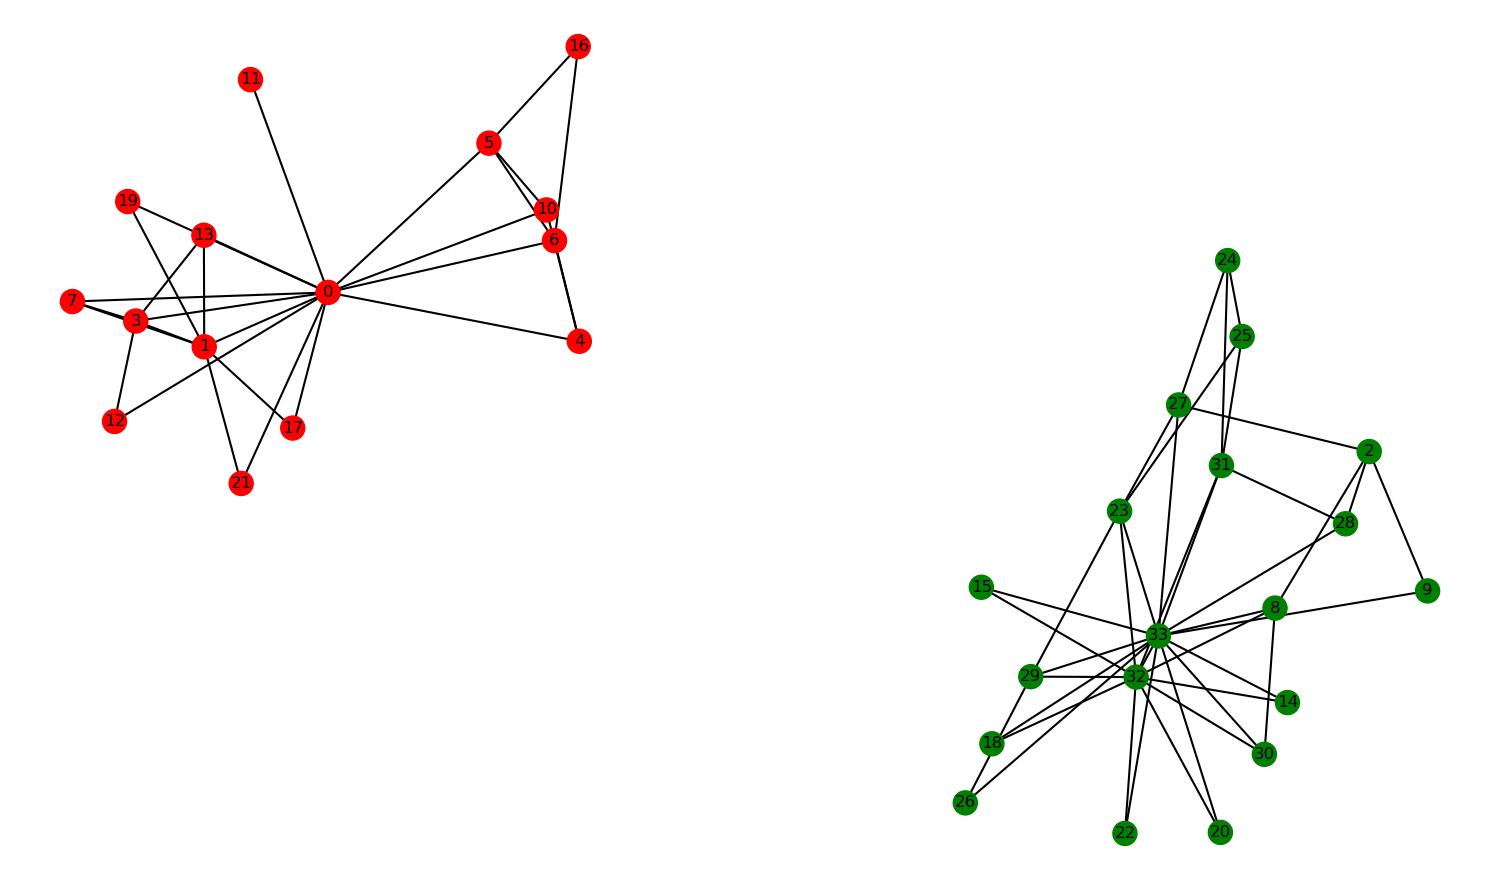
\includegraphics[trim=0 0 0 0, clip, width=170mm] {11y.PNG}
    \caption{Final split by Girvan-Newman algorithm}
    \label{fig:web-growth}
\end{figure}
\clearpage
\begin{figure}[h]
    \centering
    % trim and clip are used to crop the image, trim=left bottom right top
    % width sets max width, height will be scaled appropriately
    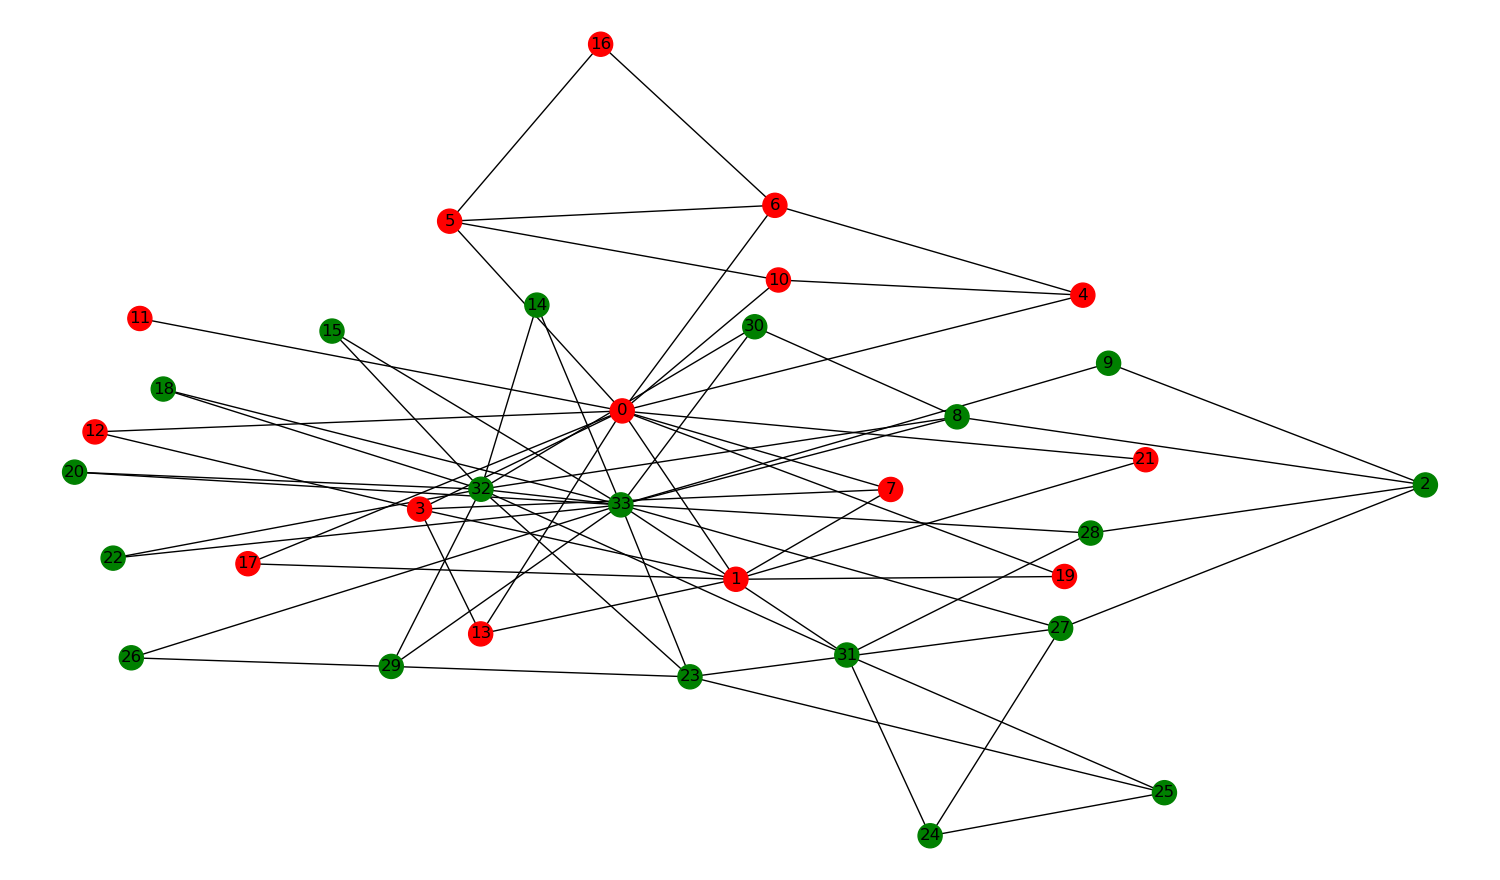
\includegraphics[trim=8 0 8 8, clip, width=170mm] {finalgroup.PNG}
    \caption{Appropriately divided node colors but edges are same}
    \label{fig:web-growth}
\end{figure}

\subsection*{Discussion}
\emph{Q: Did all of the same colored nodes end up in the same group? If not, what is different?}

Yes all the colored node ended up in the same group. The driver code for this is:

\begin{itemize}
\lstinputlisting[language=Python,caption=mygraph.py, label=Q3:import,firstnumber=114,firstline=114,lastline=120]{mygraph.py}

The component function is used to breakdown the nodes into various node colors of green and red
\lstinputlisting[language=Python,caption=Get the NodeView object separating into red and green categories, label=Q3:import,firstnumber=32,firstline=32,lastline=44]{mygraph.py}

Then launched the driver for Girvan-newman algorithm on line 118
\lstinputlisting[language=Python,caption= Girvan-newman algorithm , label=Q3:import,firstnumber=118,firstline=118,lastline=118]{mygraph.py}
        
Then found the maximum edge called it the findedge
\lstinputlisting[language=Python,caption= findedge, label=Q2:import,firstnumber=22,firstline=22,lastline=30]{mygraph.py}

Then built the edge color list and width of the edge list, to set the color coding and width variable

\lstinputlisting[language=Python,caption= Setting and reset edges color and width values, label=Q3:import,firstnumber=62,firstline=62,lastline=76]{mygraph.py}
Then plotted using the plot function and built the path for after the removal of edges
\lstinputlisting[language=Python,caption= mygraph.py, label=Q3:import,firstnumber=84,firstline=84,lastline=95]{mygraph.py}
        
\end{itemize}

\section*{Q4}
We know the group split in two different groups. Suppose the disagreements in the group were more nuanced. What would the clubs look like if they split into 3, 4, and 5 groups? A single node can be considered as a "group".

\subsection*{Answer}
\clearpage
\begin{figure}[h]
    \centering
    % trim and clip are used to crop the image, trim=left bottom right top
    % width sets max width, height will be scaled appropriately
    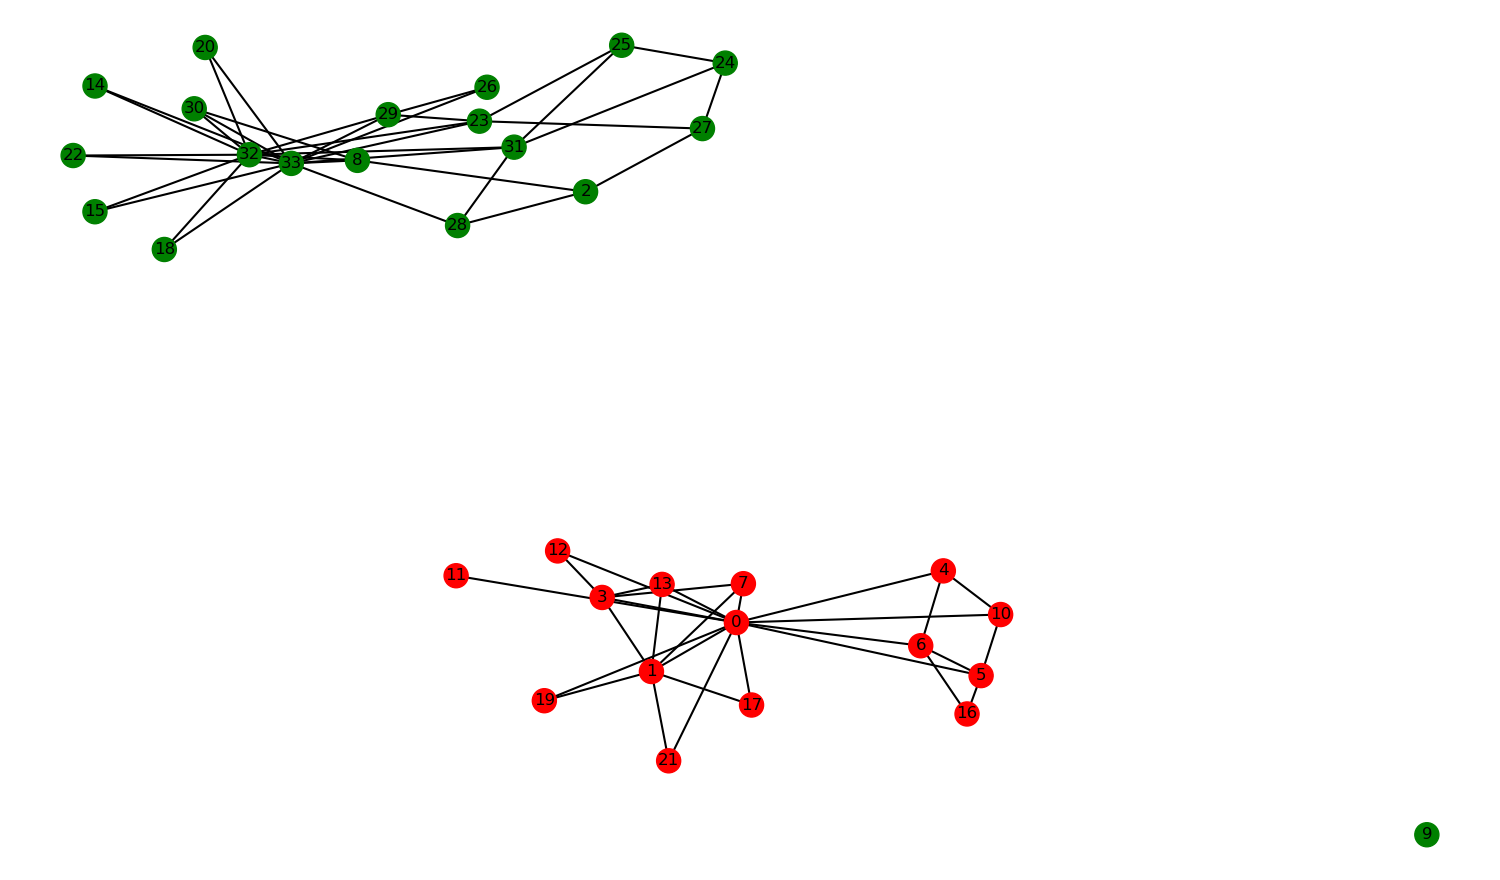
\includegraphics[trim=8 0 8 8, clip, width=160mm] {14y.PNG}
    \caption{Group 3}
    \label{fig:web-growth}
\end{figure}
\clearpage
\begin{figure}[h]
    \centering
    % trim and clip are used to crop the image, trim=left bottom right top
    % width sets max width, height will be scaled appropriately
    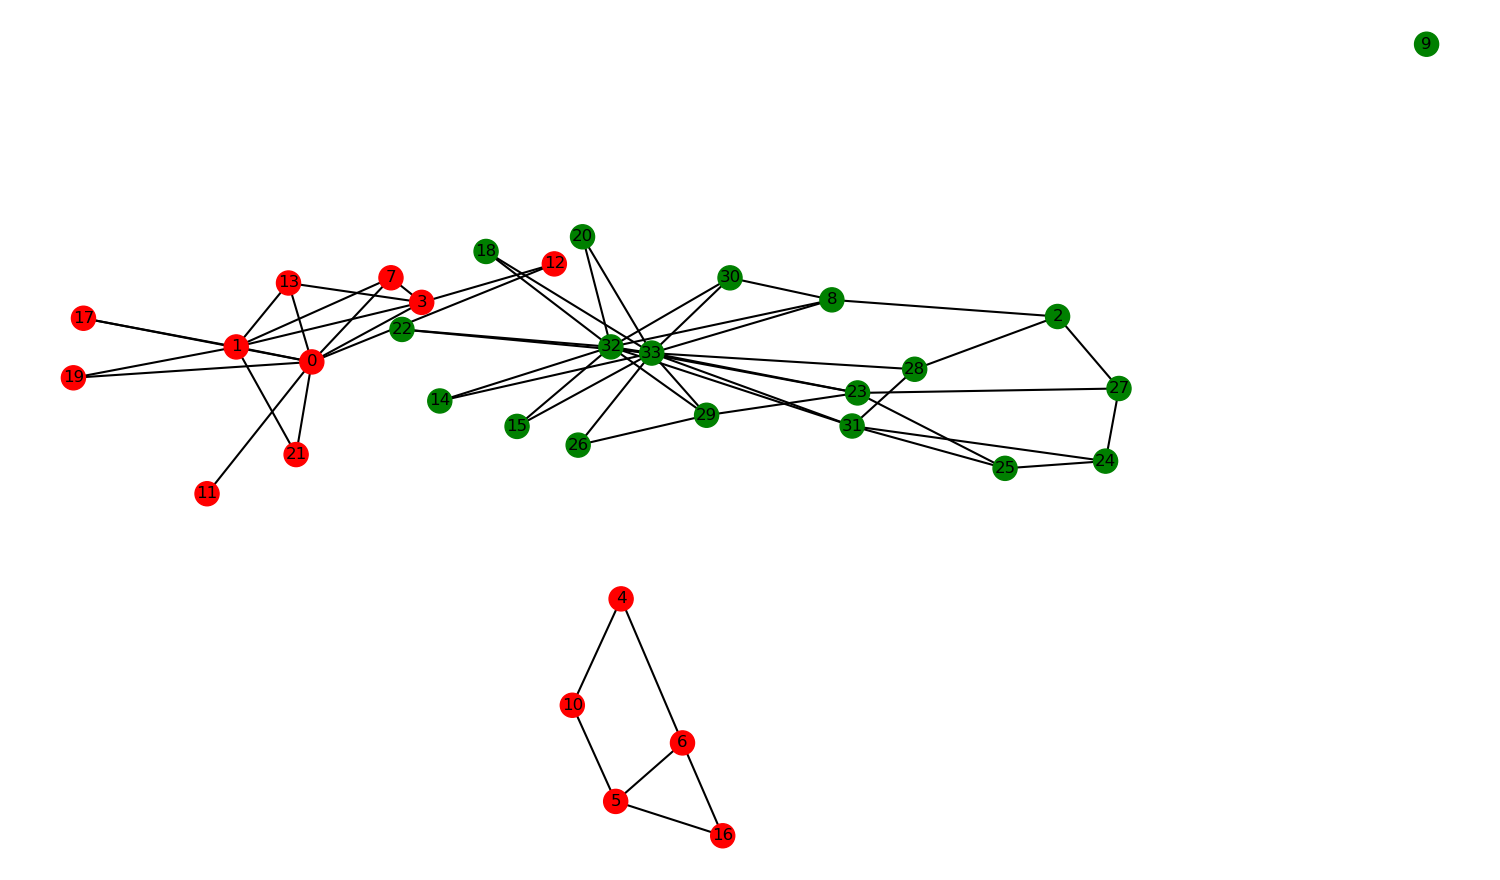
\includegraphics[trim=8 0 8 8, clip, width=170mm] {18y.PNG}
    \caption{Group 4}
    \label{fig:web-growth}
\end{figure}
\clearpage
\begin{figure}[h]
    \centering
    % trim and clip are used to crop the image, trim=left bottom right top
    % width sets max width, height will be scaled appropriately
    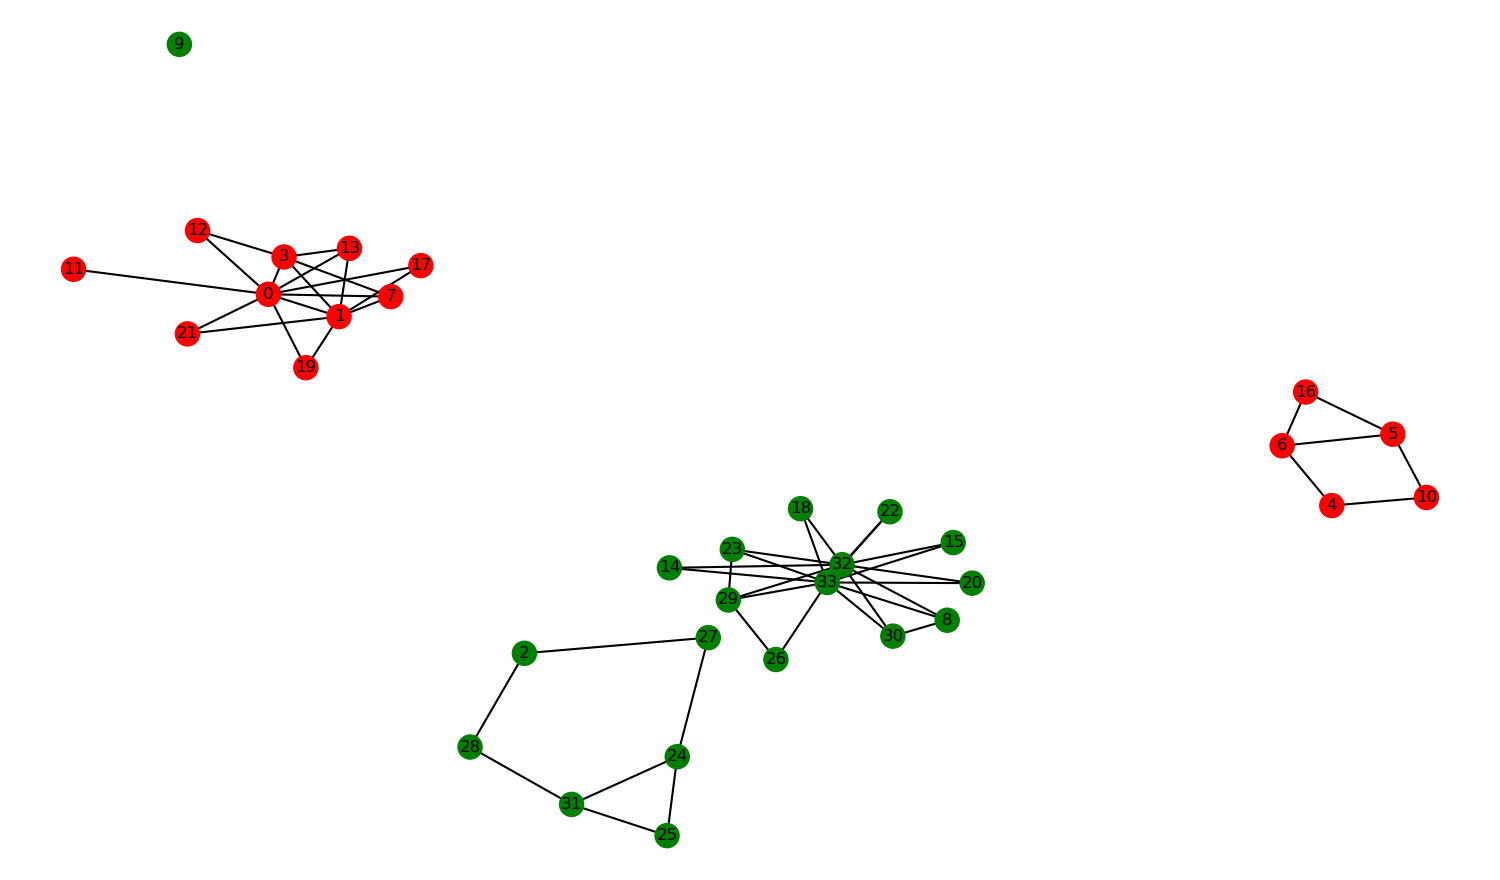
\includegraphics[trim=8 0 8 8, clip, width=170mm] {24y.PNG}
    \caption{Group 5}
    \label{fig:web-growth}
\end{figure}
\subsection*{Discussion}
The same algorithm of previous question produced these outputs. This is how the club groups would look like if they are split into 3,4 and 5 groups.

\section*{References}

\begin{itemize}
    \item {NetworkX, \url{https://networkx.org/documentation/stable/tutorial.html}}
    \item {NetworkX , \url{https://networkx.org/documentation/stable/reference/drawing.html#module-networkx.drawing.nx_pylab}}
    \item {NetworkX , \url{https://gawron.sdsu.edu/python_for_ss/course_core/book_draft/Social_Networks/Networkx.html}}
    \item {StackoverFlow,
    \url{https://stackoverflow.com/questions/332289/how-do-you-change-the-size-of-figures-drawn-with-matplotlib}}
   \item {StackoverFlow,
    \url{https://stackoverflow.com/questions/9012487/matplotlib-pyplot-savefig-outputs-blank-image}}
    \item {Girvan Newman,
    \url{https://networkx.org/documentation/stable/reference/algorithms/generated/networkx.algorithms.community.centrality.girvan_newman.html}}
   
    
\end{itemize} 



\end{document}
\end{document}
